\documentclass[twoside,11pt]{article}
\usepackage{relsize}
\usepackage{times}
%\usepackage{epsfig}
\usepackage{amsmath}
%\usepackage{amsthm}
%\usepackage{amssymb}
\usepackage{natbib}
\usepackage{graphicx}
\usepackage{epstopdf}
\usepackage{dsfont}
\usepackage{lipsum}
\usepackage{bbm}
%\usepackage{subfigure}

\usepackage{epsfig}
\usepackage{amssymb}
\usepackage{natbib}
\usepackage{graphicx}
\usepackage{jmlr2e}
\newtheorem{mydef}{Definition}
\usepackage{algorithm}
\usepackage{algorithmic}
\newcommand{\erf}[1]{\mathsf{erf}#1}
\newcommand{\dataset}{{\cal D}}
\newcommand{\fracpartial}[2]{\frac{\partial #1}{\partial  #2}}
\newcommand{\wl}{W_{\textsc{\textsc{\relsize{-2}{\textsl{LHM}}}}}}
\newcommand{\argmin}{\mathop{\mathrm{argmin}}}

\usepackage{lastpage}
\jmlrheading{19}{2018}{1-\pageref{LastPage}}{7/17; Revised
9/18}{10/18}{17-402}{Dolev Raviv,Tamir Hazan, and Margarita Osadchy}
\ShortHeadings{Hinge-Minimax Learner for the Ensemble of Hyperplanes}{Dolev Raviv,Tamir Hazan, and Margarita Osadchy}
\firstpageno{1}

\begin{document}
\title{Hinge-Minimax Learner for the Ensemble of Hyperplanes}

\author{\name Dolev Raviv \email dolev.raviv@gmail.com \\
       \addr Department of Computer Science\\
       University of haifa\\
       Haifa, 31905, Israel
        \AND
       \name Tamir Hazan \email tamir.hazan@technion.ac.il\\
       \addr Faculty of Industrial Engineering and Management\\
       Technion - Israel Institute of Technology\\
       Haifa, 32000, Israel
       \AND
       \name Margarita Osadchy \email rita@cs.haifa.ac.il\\
       \addr Department of Computer Science\\
       University of haifa\\
       Haifa, 31905, Israel}

\editor{David Sontag}
\maketitle

\begin{abstract}
In this work we consider non-linear classifiers that comprise intersections of hyperplanes. We learn these classifiers by minimizing the ``minimax'' bound over the negative training examples and the hinge type loss of the positive training examples. These classifiers fit typical real-life datasets that consist of a small number of positive data points and a large number of negative data points. Such an approach is computationally appealing since the majority of training examples (belonging to the negative class) are represented by the statistics of their distribution, which is used in a single constraint on the empirical risk, as opposed to SVM, in which the number of variables is equal to the size of the training set. We first focus on intersection of $K$ hyperplanes, for which we provide empirical risk bounds. We show that these bounds are dimensionally independent and decay as $K/\sqrt{m}$ for $m$ samples. We then extend the K-hyperplane mixed risk to  the latent mixed risk for training a union of $C$ $K$-hyperplane models, which can form an arbitrary complex, piecewise linear boundaries.  We propose efficient algorithms for training the proposed models.
Finally, we show how to combine hinge-minimax training with deep architectures and extend it to multi-class settings using transfer learning. The empirical evaluation of the proposed models shows their advantage over the existing methods in a small training labeled data regime.
\end{abstract}

\begin{keywords}
  Minimiax, Imbalanced Classification, Intersection of K Hyperplanes, Transfer Learning
\end{keywords}

\section{Introduction}
Many real-life binary classification problems involve imbalanced classes, for example object detection in vision and fraud detection in security.  In such problems it is easy to collect background data (the negative class), while data representing the target class (the positive class) is rare or hard (expensive) to obtain. The majority of existing classifiers (e.g., SVM, Neural Networks, including deep ones) assume balanced training sets and when trained on imbalanced sets show degraded classification performance or require a long and tedious bootstrapping process of mining negative examples (e.g.~\cite{eSVM,ROSS}) out of millions.

When there are (infinitely) many training examples, instead of minimizing the average sample loss, it is more computationally appealing to apply minimax setting  (\cite{Lanckriet2003,Honorio14}), which upper bounds the expected risk of a classifier assuming only the knowledge of  mean and covariance of the data distribution. The ``minimax'' bound provides an upper bound for \emph{every} distribution with a given mean and covariance. Applying the minimax learning (\cite{Lanckriet2003}) to the negative class (the majority class) allows to avoid bootstrapping procedure and makes learning more efficient, as it replaces loss evaluation on all negative samples with a single ``minimax'' bound.

Due to the assumption that the positive class is rare, we cannot apply the minimax learning to the positive class, as it completely relies on the mean and covariance of the data. Estimating the covariance matrix in high-dimensional space from a small number of positive training samples is problematic.  Alternatively, we can use the hinge loss (\cite{Vapnik00,Zhang02,Bartlett03,Bousquet04,Kakade08}) for the positive class as it is computationally appealing when there are fairly small number of training samples.


We suggest to combine the hinge-like loss for the positive samples with the ``minimax'' bound applied to the statistics of the negative samples to enjoy the best of both worlds and we call these classifiers \emph{Hinge-Minimax} classifiers.

The idea of combining ``minimax'' bound for the negative class and svm-like formulation for the positive samples was introduced in \cite{OsadchyKF12,OsadchyKR16} for computing linear and kernel classifiers. Kernel classifiers could be quite slow, as they require evaluating kernel on many support vectors.  In this work we focus on more efficient non-linear classifiers -- ensembles of hyperplanes. We first consider an intersection of hyperplanes and then extended it to more general ensembles of hyperplanes.


Previous algorithms for intersection of hyperplanes are computationally costly when considering large sets of negative data points (\cite{Klivans09,DanielyLS14}). To deal with this computational difficulty we use the mixed risk. Namely, we extend the ``minimax'' bound to deal with intersection of hyperplanes over (infinitely many) negative examples. %As this risk bound is loose when there are few data points, as we have in the positive set,
For the positive samples, we define a K-hyperplane hinge loss. We derive an empirical mixed-risk bound, that uses the Rademacher complexities to bound the risk of the positive class and vector Bernstein's inequalities to bound the risk associated with the negative class. Note that we treat the positive and negative samples differently because of the computational gain such separation provides.

Recently,~\cite{Honorio14} derived a generalization bound for the minimax setting using PAC-Bayesian approach, which bounds the expected loss with respect to a posterior distribution over all possible classifiers. Our work differs as we use stronger assumptions - that the norm of the data points is bounded by a constant, an assumption that is natural in many applications.\footnote{Input normalization is a standard procedure, applied for faster learning.} Thus we are able to avoid the PAC-Bayesian approach that considers generalization bounds over randomized predictors. %Instead we use Rademacher complexity to derive generalization bounds for deterministic predictors.


Intersection of positive half-spaces is a convex set. We generalize the mixed risk for a non-convex classifier.  We learn an ensemble of K-hyperplane models, that can form arbitrary, piece-wise linear boundaries. We propose a training algorithm that minimizes this risk by simultaneously discovering the convex components in the positive class and building K-hyperplane models to separate each component from the negative class. The learning is done by alternating between finding the best partition of the data into hidden components and updating the model over this partition. We call this novel classifier the \emph{Latent Hinge Minimax} (LHM) classifier, as it discovers the latent structure in the data and employs the Hinge-Minimax paradigm.



We show that the LHM model has an equivalent Neural Networks (NN) architecture. This allows us 1) to use deep learning features via transfer learning and 2) to extend the proposed model to the multi-class setting. For the multi-class problems, we build one-against-all classifiers for all classes and combine them in a single model by mapping class specific LHM models to a multi-class NN with a matching architecture. We then use the cross-entropy loss to adjust the weights in the resulting \emph{LHM-NN} combination.

We show that using LHM-NN in the transfer learning settings has significant benefits compared to NN (standard settings), in both classification accuracy and training efficiency. The improved accuracy stems from the ability of LHM model to learn from unlabeled data. The fast convergence of the LHM-NN (just a handful of epochs) is due to a very good initialization of the upper layers with class specific LHM classifiers. Note that class specific LHM models can be trained in parallel. Moreover, adding a new class to LHM-NN is fast and easy: train a classifier for the new class, map it to the corresponding LHM-NN architecture and run a very fast fine-tuning. Similarly to \cite{fromNtoN+1}, which considered the transfer learning for the $n+1$ category from a fully trained $n$-category classifier, we use only a handful of training samples for tuning it. In contrast to \cite{fromNtoN+1}, we do not restrict the new classifier to belong to the span of the previously learned $n$ classifiers. This allows us greater flexibility in adding a new, non-related class to the multi-class model.


We performed empirical evaluation of the proposed models: the K-hyperplane, the LHM, and the multi-class models. In all cases, the proposed models outperformed their counterparts in small and imbalanced training data regime.

The rest of the paper is organized as follows.
Section 2 introduces the  K hyperplane Hinge-Minimax classifier (KHHM). Specifically, we extend the  ``minimax'' bound for the intersection of K positive half-spaces in Section 2.1.1. Then in Section 2.2, we propose a novel training algorithm for the KHHM classifier. We prove the uniform generalization bounds for the KHHM model in Section 2.3.  Section 3 focuses on a non-convex generalization of the KHHM model -- LHM classifier. We introduce the latent mixed risk in Section 3.1, the training algorithm in Section 3.2, and we prove a uniform generalization bound for the LHM classifier with a fixed assignment of the positive labeled training set in Section 3.3. Section 4 discusses the mapping of the LHM classifier to a neural network. Section 5 reports the experiments with KHHM, LHM, and LHM-NN classifiers. Section 6 discusses the efficiency of the proposed models and Section 7 concludes the paper.

\section{K-Hyperplane Hinge-Minimax Classifier}
In the following, for simplicity  we assume that for a linear classifier which predicts $y=sign(w^Tx)$, $b=0$ (or absorbed by $w$).

\begin{mydef} Let $w_i$, $i=1,..,K$ denote $K$ hyperplanes. Let $W$ be a matrix with $w_i$ as its $i$th column. We define K-hyperplane classifier $f_W(x)$ as an intersection of these $K$ half-spaces:
\begin{equation}\label{eq_non_linear_classifier}
 f_W(x)=\left\{
              \begin{array}{ll}
              1 & \mbox{if  } W^\top x \geq \vec{0} \\
              -1 & \mbox{otherwise} \\
              \end{array}
          \right.
 \end{equation}
 where $\vec{0}$ denotes a vector of zeros.
\end{mydef}
\subsection{Mixed Risk for K-Hyperplane Model}\label{KHHM}
We are interested in a classification problem in which the positive class corresponds to a single concept and the negative class is its complement and we refer to it as a \emph{background}. We assume that the sample of the positive class is relatively small while the negative sample is very large (it can be represented by an unlabeled data as well, thus is easy to collect). Due to the specifics of the problem we propose a mixed risk for the non-linear classifier in eq. \ref{eq_non_linear_classifier}. We first define its parts in Definitions 2 and 3 and then define the mixed risk in Definition 4.
\begin{mydef} Let $(x,y)\sim D$  be a joint distribution of samples $x \in \mathbb{R}^n$ and labels $ y \in \{-1,1\}$.
We define the \emph{hinge risk} of $f_W(x)$ as follows,
\begin{equation}
\label{def_hinge_risk}
L_D^{H}(W)=\mathbb{E}_D\left[\ell(W,x,y)\mathbbm{1}[y=1]+0\cdot \mathbbm{1}[y=-1]\right]
\end{equation}
where $\ell(W,x,y)=\max_{j\in\{1,...,K\}} \{\max\{0,1-yw_j^\top x\}\}$.
\end{mydef}

\begin{mydef}
Under the assumptions of Definition 2, let $D_{neg}$ be a marginal distribution of samples from a ball of radius $C$ over the negative labels  with mean $\mu$ and covariance matrix $\Sigma$.  Let $\Omega(\mu,\Sigma)$ be a family of all distributions with mean $\mu$ and covariance matrix $\Sigma$. We assume that $D_{neg}\in \Omega(\mu,\Sigma)$.

We define the \emph{background risk}\footnote{the name ``background'' is chosen to emphasize the fact that the negative class is the majority class, while the positive class is rare.} of  $f_W(x)$ as follows,
\begin{equation}
L^{B}_{\mu,\Sigma}(W)=\left[\sup_{Z\in\Omega(\mu, \Sigma)}Pr_{z\sim Z}(W^\top z\geq\vec{0})\right]\mathbbm{1}[y=-1]+0\cdot \mathbbm{1}[y=1]
\end{equation}
\end{mydef}
We derive the expression for the background risk in the next section.

According to the Definitions 2 and 3, the hinge risk is defined over the samples of the positive class only and the background risk is defined over the distribution of the negative class only. Thus we can sum the two to form the mixed risk over $D$.

\begin{mydef} Under the assumptions of Definitions 2 and 3,
we define the mixed risk for the K-hyperplane classifier as:
\begin{equation}\label{eq_risk}
L^{HB}_D(W)=L_D^{H}(W)+L^{B}_{\mu,\Sigma}(W),
\end{equation}
\end{mydef}


\subsubsection{The Expected Risk of the Negative Class}\label{subsection_k_minimax_risk}

The extension of Theorem 3.1 from ~\cite{marshall1960} to a nonzero mean variable (as shown in ~\cite{marshall1960} Eq. 7.7--7.8) states that for a random vector $x$ with mean $M$ and covariance $\Gamma$,
\[
\sup_{x\sim (M, \Gamma)}\Pr(x\in S)=\frac{1}{1+d^2},
\]  with $d^2=\inf_{x\in S}(x-M)^\top  \Gamma^{-1}(x-M),$
where S is a given convex set.

The intersection of $K$ hyperplanes is a convex set, thus we can bound the probability of a negative sample falling into the intersection of $K$ hyperplanes using the above result and derive the expression for $L^{B}_{\mu,\Sigma}(W)$ as shown below in Theorem~\ref{th_risk}.

%Since $L^{M}_{\mu,\Sigma}(W)$ is the risk of a negative sample falling into the intersection of $K$ hyperplanes, which is a convex set, we can use the theorem due to ~\cite{marshall1960} to derive the expression for  $L^{M}_{\mu,\Sigma}(W)$.


\begin{theorem}
\label{th_risk}
%Let $Z(\mu, \Sigma)$ be all distributions with known mean $\mu$ and covariance $\Sigma$. %For $K$ fixed hypeplanes $w_j$ $(j=1,..,K)$,
For any finite number of hyperplanes $w_j$,
$$\sup_{Z\in\Omega(\mu, \Sigma)}Pr_{z\sim Z}(W^\top z\geq\vec{0})=\frac{1}{1+d^2}$$
with $d^2=\mu^\top U(U^\top \Sigma U)^{-1}U^\top\mu,$
where $U$ is a subset of columns of $W$ that satisfy $w^\top z^*=0$,
where $z^*=\arg\min_z(z-\mu)^\top \Sigma^{-1}(z-\mu).$
\end{theorem}
\begin{figure}[t]
\center{
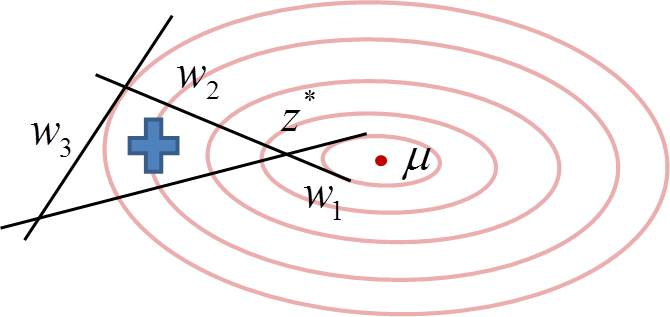
\includegraphics[width=2.5in]{ex_2d_wedge.jpg}
\caption {A 2D illustrative example of Theorem \ref{th_risk}. $z^*$ is the closest point to the mean of the negative distribution.}
}\label{ex_il}
\end{figure}
Before we proceed with the proof, let us consider the following 2D toy example to gain some intuition into Theorem \ref{th_risk} (see Figure \ref{ex_il}). Assume that the positive class lies inside an intersection of three hyperplanes $W=[w_1, w_2, w_3]$ and the negative class is described by the normal distribution with mean $\mu$ and covariance $\Sigma$. $d^2$ is a square distance between the mean of the negative distribution and the point on the boundary of the positive region of the classifier, which is closest to $\mu$. In the example, depicted in Figure \ref{ex_il},  the closest point is denoted by $z^*$ and it's an intersection of $w_1$ and $w_2$, thus  $U=[w_1,w_2]$.

\begin{proof}
Let $z\sim D_{neg}\in\Omega(\mu,\Sigma)$ be a sample from the negative class. $W^\top z \geq \vec{0}$ defines a convex set, thus we can apply the result due to ~\cite{marshall1960} to obtain:
\[
\sup_{Z\in\Omega(\mu, \Sigma)}Pr_{z\sim Z}(W^\top z\geq \vec{0})=\frac{1}{1+d^2},
\]  with $d^2=\inf_{W^\top z\geq \vec{0}}(z-\mu)^\top  \Sigma^{-1}(z-\mu),$
where the supremum is taken over all distributions in $\Omega(\mu,\Sigma)$.

Next, we want to derive a closed-form expression for $d^2$.
We seek the solution for the primal problem
\[
\min_{z}(z-\mu)^\top \Sigma^{-1}(z-\mu)
\]
s.t. $w_i^\top z\geq 0$ for $i=1,..,K.$
We construct the Lagrangian:
$$L(z,\lambda_i)=(z-\mu)^\top  \Sigma^{-1}(z-\mu)+\sum_i \lambda_i w_i^\top z, \;\; \lambda_i\geq0.$$
The optimality condition:
$$\frac{\partial L}{\partial z}=2\Sigma^{-1}z - 2\Sigma^{-1}\mu
+\sum_i\lambda_iw_i=0,$$
gives us
$z^*=\mu-\frac{1}{2}\sum_i\lambda_i\Sigma w_i.$
The Lagrange dual function is as follows,
\begin{equation}\label{eq_dual_func}
L(z^*,\lambda)=\left(\frac{1}{2}\sum_i \lambda_i \Sigma w_i\right)^\top \Sigma^{-1} \left(\frac{1}{2}\sum_j\lambda_j\Sigma w_j\right) +\sum_i\lambda_iw_i^\top \left(\mu-\frac{1}{2}\sum_j\lambda_j\Sigma w_j\right)
\end{equation}
%\begin{flalign}\label{eq_dual_func}
%&L(z^*,\lambda)=\left(\frac{1}{2}\sum_i \lambda_i \Sigma w_i\right)^\top %\Sigma^{-1}\left(\frac{1}{2}\sum_j\lambda_j\Sigma w_j\right)\\ \nonumber &+\sum_i\lambda_iw_i^\top %\left(\mu-\frac{1}{2}\sum_j\lambda_j\Sigma w_j\right)
%\end{flalign}
The optimality conditions are:
$$\frac{\partial L(z^*,\lambda)}{\partial \lambda_t}=-\frac{1}{2}\sum_i\lambda_iw_t^\top \Sigma w_i+w_t^\top \mu=0$$
for $t$ such that $\lambda_t>0$.

\noindent The function is optimized at
\begin{equation}\label{req_lambda_opt}
\lambda^*=2(U \Sigma U)^{-1}U^\top \mu,
\end{equation}
where $U$ is formed by a subset of columns of $W$ for which $\lambda_t>0$, and thus $w_t^\top  z^*=0$.

For the last step we substitute the optimal $\lambda$, given in eq. \ref{req_lambda_opt} into the dual function in eq. \ref{eq_dual_func} and after simple algebraic manipulations we get:

\begin{equation*}
d^2=\max_{\lambda\geq 0}(L(z^*,\lambda^*))=\mu^\top U(U^\top  \Sigma U)^{-1}U^\top \mu
\end{equation*}
\end{proof}

Given the result of Theorem~\ref{th_risk}, we can express the background part of the mixed risk of the K-hyperplane classifier as follows,
$$L^{B}_{\mu,\Sigma}(W)= \sup_{Z\in \Omega(\mu, \Sigma)}Pr_{z\sim Z}(W^\top z\geq\vec{0})= \frac{1}{1+\mu^\top U(U^\top  \Sigma U)^{-1}U^\top \mu}$$

\subsection{K-Hyperplane Hinge-Minimax (KHHM) Training} \label{KHHM_Alg}
We aim to minimize the mixed risk in eq. \ref{eq_risk}. To this end, we minimize the empirical risk
\begin{equation}
\label{eq_emp_risk}
L^{HB}_S=L_S^{B}(W)+L_S^{H}(W)
\end{equation}
regularized by the sum of $L_2$ norms of the $K$ hyperplanes: $\frac{C}{2}\sum_i\|w_i\|^2 + L^{HB}_S$.  This empirical risk is a non convex and non smooth function, hence a gradient based optimization of it is difficult. However, \cite{OsadchyKR16}  showed an algorithm for approximating this problem for a single hyperplane $\mathbf{w}$ using the following convex formulation:
%\begin{equation}
%\begin{aligned}
%\underset{\mathbf{w},\xi}{\text{minimize}}
%&\;\;\|\mathbf{w}\|^2+C\sum_{i=1}^n\xi_i\\
%\text{subject to}
%&\;\;\mathbf{w}\cdot\mathbf{x}_i \geq1-\xi_i,\\
%&\;\;\xi_i\geq 0,\\
%&\;\;\gamma\sqrt{\mathbf{w}^T\Sigma_x\mathbf{w}}+\mathbf{w}^T\bar{\mathbf{x}}
%\leq 0.
%\end{aligned}\label{linear_opt}
%\end{equation}
\begin{equation}
\begin{aligned}
\underset{\mathbf{w}}{\text{minimize}}
&\;\;\lambda\|\mathbf{w}\|^2+\sum_i \max\{0,1-\mathbf{w}^\top x_i\}\\
\text{subject to}
&\;\;\gamma\sqrt{\mathbf{w}^\top\Sigma\mathbf{w}}+\mathbf{w}^\top\mu\leq 0.
\end{aligned}\label{linear_opt}
\end{equation}
where $\gamma=\sqrt{\frac{1-\delta}{\delta}}$. This formulation minimizes the regularized hinge loss on the positive samples while constraining the probability of ``background'' data misclassified by the classifier $\mathbf{w}$ to be less than a small threshold $\delta$.

We approximate the solution to the problem in eq. \ref{eq_emp_risk} by finding K hyperplanes $W$, which minimize the regularized hinge loss $L_S^{H}(W)$ on the positive samples while constraining the probability of ``background'' data misclassified by the intersection of these hyperplanes to be less than a small threshold $\epsilon$.

We propose an algorithm (Algorithm 1) that computes the hyperplane iteratively, each hyperplane at a time using~\cite{OsadchyKR16}. Note that since the algorithm in~\cite{OsadchyKR16} constraints  the supremum over all distributions with given $\mu$ and $\Sigma$, it constraints an upper bound on the true distribution of the negative class. However, for a Gaussian distribution the bound is tight.

The Algorithm 1 starts by training $K$ hyperplanes in a greedy manner and then iteratively adjusts each hyperplane to further reduce the loss.
%\begin{algorithm}
% \begin{algorithmic}
% \caption{KHHM Training}
% \STATE \textbf{Input:} $\{x_i\}, i=1,..,m^+$ a set of positive examples; $\{z_i\}, i=1,..,m^-$ a set of negative examples.
% \STATE \textbf{Output:} $W$ ($K$ hyperplanes)
% \STATE
% \COMMENT{The initial greedy step}
% \STATE Estimate  $\mu$ and $\Sigma$ using $\{z_i\}_i^{m^-}$
% \STATE Find $w_1$ using~\cite{OsadchyKR16}  with $\mu$ and $\Sigma$.
% \FOR{t=2 to k}
%    \STATE  Estimate  $\mu_t$ and $\Sigma_t$ using $\{z_i\mid w_j^\top z_i>0, j=1,..,t-1 \}$
%   \STATE Find $w_t$ using ~\cite{OsadchyKR16} with $\mu_t$ and $\Sigma_t$.
% \ENDFOR
% \STATE
% \COMMENT{The refinement iterations}
% \STATE Let $P_t$ be the probability $Pr(W^\top z>0)$ in iteration $t$
% \WHILE{ ($P_{t-1}-P_t>\epsilon$)}
%   \STATE Estimate  $\mu_t$ and $\Sigma_t$ using $\{z_i\mid w_j^\top z_i>0, j=1,..,K; j\neq t \}$.
%   \STATE Find $w_t$ using~\cite{OsadchyKR16} with $\mu_t$ and $\Sigma_t$.
% \ENDWHILE
% \end{algorithmic}
% \end{algorithm}
\begin{algorithm}
 \begin{algorithmic}
 \caption{KHHM Training}
 \STATE \textbf{Input:} $\{x_i\}, i=1,..,m^+$ a set of positive examples; $\{z_i\}, i=1,..,m^-$ a set of negative examples.
 \STATE
 \STATE \textbf{Initialization:} \\\hspace{0.5cm} Estimate  $\mu$ and $\Sigma$ using $\{z_i\}_i^{m^-}$. Find $w_1$ using~\cite{OsadchyKR16}  with $\mu, \Sigma$.\\\hspace{0.5cm}
     \textbf{for } {t=2 to k} \textbf{do} \\\hspace{1cm}
        Estimate  $\mu_t$ and $\Sigma_t$ using $\{z_i\mid w_j^\top z_i>0, j=1,..,t-1 \}$\\\hspace{1cm}
        Find $w_t$ using ~\cite{OsadchyKR16} with $\mu_t$ and $\Sigma_t$. \\\hspace{0.5cm}
     \textbf{end for}
     %\ENDFOR
 \STATE
 \STATE \textbf{Training:}\\\hspace{0.5cm}
 \textbf{for } {t=$1,2,3...$} \textbf{do} \\\hspace{1cm}
   Let $P_t$ be the probability $Pr(W^\top z>0)$ in iteration $t$\\\hspace{1cm}
   \textbf{if }($P_{t-1}-P_t>\epsilon$)\\\hspace{1.5cm}
      Estimate  $\mu_t$ and $\Sigma_t$ using $\{z_i\mid w_j^\top z_i>0, j=1,..,K; j\neq t \}$.\\\hspace{1.5cm}
      Find $w_t$ using~\cite{OsadchyKR16} with $\mu_t$ and $\Sigma_t$.\\\hspace{1cm}
   \textbf{else }\\\hspace{1.5cm}
   \textbf{Output} $W$ ($K$ hyperplanes)\\\hspace{1cm}
   \textbf{end if}\\\hspace{0.5cm}
   \textbf{end for}
%  \FOR{$t=1,2,3,...$}
% \STATE Let $P_t$ be the probability $Pr(W^\top z>0)$ in iteration $t$
% \IF{ ($P_{t-1}-P_t>\epsilon$)}
%   \STATE Estimate  $\mu_t$ and $\Sigma_t$ using $\{z_i\mid w_j^\top z_i>0, j=1,..,K; j\neq t \}$.
%   \STATE Find $w_t$ using~\cite{OsadchyKR16} with $\mu_t$ and $\Sigma_t$.
% \ELSE
% \STATE Output $W$ ($K$ hyperplanes)
%  \ENDIF
% \ENDFOR
 \end{algorithmic}
 \end{algorithm}
 \begin{lemma}
   Algorithm 1 minimizes the regularized hinge loss $L_S^{H}(W)$ on the positive samples while keeping $Pr(W^\top z\geq \vec{0})\leq \epsilon$ (for a small $\epsilon$).
 \end{lemma}

\begin{proof}
Let $Z$ denote the distribution of the negative class and $z\sim Z$ denote a sample from this distribution.  Let $S^t$ denote the  part of negative class that falls inside the intersection of $K-1$ hyperplanes ($w_t$ is not included): $$S^t= \{z|w_i^\top z\geq 0, \forall i \in \{1,...,K\}\setminus\{t\} \}.$$
%Let $Z^t$ denote a distribution in the intersection of $K-1$ hyperplanes ($w_t$ is not included) .
In step i, Algorithm 1 finds $w_{t_i}$ that minimizes the hinge loss (which is always positive) of $w_{t_i}$ over positive labels and constrains  $Pr(w_{t_i}^\top z \geq 0)| z \in S^{t_i})\leq \delta$, while keeping the rest of the hyperplanes fixed.

The empirical risk of the intersection of $K$ hyperplanes over positive labels is the maximum over $K$ of hinge losses. Thus, the hinge loss of $W$ is decreased at the iterations, in which the hyperplane with the maximal loss is updated, and it remains unchanged otherwise. Consequently,  Algorithm 1  minimizes the hinge loss of $W$.

We can write
$$Pr(W^\top z \geq 0)=Pr(w_{t_i}^\top z \geq 0)| z \in S^{t_i})Pr(z \in S^{t_i})+ 0\cdot Pr(z\notin S^{t_i}).$$
$Pr(z \in S^{t_i})=a$ which is constant (does not depend on $w_{t_i}$) and $Pr(w_{t_i}^\top z \geq 0)| z \in S^{t_i})\leq \delta$. Thus, $Pr(W^\top z \geq 0)\leq a\delta $. Setting $\epsilon=a\delta$ concludes the proof.
\end{proof}



\subsection{Generalization Bound for KHHM Model}
\label{sec:khhm_bond}
In the following we bound the mixed risk of the KHHM classifier by its finite sample. We show that the discrepancy between the risk $L^{HB}_D(W)$ and its empirical estimation $L^{HB}_S(W)$ decays at the rate of $O(K \sqrt{\frac{\log (1/\delta)}{m}})$ where $\delta$ is the confidence over the samples of the training data and $m$ is the training data size. The main difficulty in deriving a generalization bound arises from mixing the hinge risk for the positive examples and the background risk for the negative examples. We approach this problem by deriving the uniform generalization bounds separately for the positive and negative classes.

\subsubsection{Uniform generalization bound for the empirical background risk}

Recall that $D_{neg}$ is the distribution of the negative data points, and $\mu$ and $\Sigma$ are its mean and covariance respectively. Let $\hat \mu$ and $\hat \Sigma$ be the mean and covariance estimates from the training data points that are associated with negative labels. We bound the background risk by its training sample estimation. The  generalization bound is dominated by the discrepancy
\begin{equation*}
\Delta=L^{B}_{\mu,\Sigma}(w) - L^{B}_{\hat \mu, \hat \Sigma}(w)
\end{equation*}
To provide uniform generalization bound to the background risk, we show that the discrepancy $\Delta$ decreases when the size of the training sample increases. Therefore we represent the discrepancy with $\|\hat \mu - \mu\|$ and $\|\hat \Sigma - \Sigma\|$ that decrease as a function of the training sample.

Let $U$ denote a subset of columns of $W$ that satisfy $w^\top z^*=0$, where $z^*=\arg\min_z(z-\mu)^\top \Sigma^{-1}(z-\mu)$. We make two additional assumptions on $U$: First, the number of hyperplanes $K_U$ comprising $U$ is smaller than the dimension of the features and second, the  hyperplanes in $U$ are linearly independent. Both assumptions hold in practice. The number of hypeplanes must be  small to make the classifier computationally efficient and $K_U\leq K$ (while the dimension of the feature space is usually large). The same reason justifies the independence assumption, as linearly dependent hyperplanes are redundant and do not contribute to the classifier, thus should be removed/avoided.

Using the result of Theorem 1, we can write the discrepancy $\Delta$ as follows:
\small
$$\Delta=\frac{1}{1+\mu^\top U(U^\top\Sigma U)^{-1}U^\top\mu}-\frac{1}{1+\hat{\mu}^\top U(U^\top\hat{\Sigma} U)^{-1}U^\top\hat{\mu}}$$
By noting that the denominator of both terms is greater than 1 we can upper bound $\Delta$ by omitting the denominator. Then,
$$\Delta\leq \hat{\mu}U(U^\top\hat{\Sigma}U)^{-1}U^\top\hat{\mu}-\mu^\top U(U^\top \Sigma U)^{-1}U^\top\mu $$
Next, we denote $A\triangleq U(U^\top\Sigma U)^{-1}U^\top$ and $\hat{A}\triangleq U(U^\top\hat{\Sigma } U)^{-1}U^\top$. By adding and subtracting $\mu^\top A\hat{\mu}$ and rearranging the terms, we obtain
\begin{equation}
\label{eq:Delta}
\Delta\leq\mu^\top A(\hat{\mu}-\mu)+\hat{\mu}^\top(\hat{A}-A)\hat{\mu}+(\hat{\mu}-\mu)^\top A\hat{\mu}.
\end{equation}
Denote
$$\Delta_1 \triangleq \mu^\top A(\hat{\mu}-\mu)+(\hat{\mu}-\mu)^ \top A\hat{\mu}$$ and
$$\Delta_2\triangleq \hat{\mu}^\top(\hat{A}-A)\hat{\mu}.$$ Going back to the original notations, we obtain
\begin{equation}\label{eq_D1}
\Delta_1=\mu^\top U(U^\top\Sigma U)^{-1}U^\top(\hat{\mu}-\mu)+(\hat{\mu}-\mu)^\top U(U^\top\Sigma U)^{-1}U^\top\hat{\mu}
\end{equation}
\begin{equation}\label{eq_D2}
\Delta_2=\hat{\mu}^\top(U(U^\top\hat{\Sigma } U)^{-1}U^\top-U(U^\top\Sigma U)^{-1}U^\top)\hat{\mu}
\end{equation}
In the following, let $\|\cdot\|_F$  denote the Frobenius norm of a matrix (the $\ell_2-$ norm of matrix vectorized form).
\begin{lemma}
\label{lemma:d1}
Assume $x \sim D_{neg}$ is a distribution over data points $x$ with negative labels such that $\|x\| \le C$ holds with probability $1$. Denote by $\mu$ its mean and by $\Sigma$ its covariance. Let $S_1$ denote a training sample of size $m_1$ and let $\hat \mu = \frac{1}{m_1} \sum_{x \in S_1} x$ be its sampled mean and $\hat \Sigma = \frac{1}{m_1} \sum_{x \in S_1} (x-\hat \mu) (x - \hat \mu)^\top$ be its sampled covariance. Define $\Delta_1$ as in eq. \ref{eq_D1}, where matrix $U$ has $K_U$ linearly independent columns ($K_U\leq n$) .
Assume that the minimal eigenvalues of $\Sigma, \hat \Sigma$ are lower bounded by $ \alpha  = \lambda_{min} (\Sigma), \hat \alpha  = \lambda_{min} (\hat \Sigma)$, respectively. Then, with probability at least $1-\delta$ over the draws of the training set $S_1$, the following holds uniformly for all $W$
$$\Delta_1 \le \frac{2C}{\alpha}\sqrt{\frac{32C^4 (\log (1/\delta) + 1/4)}{m_1}}$$
\end{lemma}
\begin{proof}
First, we show the upper bound
\begin{equation}
\label{eq:U_bound}
\|U(U^\top \Sigma U)^{-1}U^\top\| \leq \frac{1}{\alpha}
\end{equation}
%Let $U=V^\top S T$ be the SVD decomposition of $U$.
Following the assumption that the columns of $U$ are linearly independent and that their number is smaller than the dimension of the feature space, we can derive that
$U=\sum_{i=1}^{K_U} s_i v_i t_i^\top$, where $v_1,...,v_{K_U}$ are left singular vectors, $t_1,...,t_{K_U}$ are right singular vectors, and $s_1,...,s_{K_U}$ are singular values of $U$ which are all non-zero. %Denoting $V$ to be a tall matrix with $v_1,...,v_{K_U}$ as its columns, $T$ to be a square with $t_1,...,t_{K_U}$  as its columns, and $S$ to be a diagonal with  $s_1,...,s_{K_U}$ on the diagonal, we obtain:
Let $V$ be $n\times {K_U}$ matrix of left singular vectors $v_1,...,v_{K_U}$, $T$ be a $K_U\times K_U$ matrix of right singular vectors $t_1,...,t_{K_U}$, and $S$ be a $K_U\times K_U$ diagonal matrix of singular values $s_1,...,s_{K_U}$, then
\begin{equation}
\label{e*}
U(U^\top \Sigma U)^{-1}U^\top=VST^\top(TSV^\top\Sigma VST^\top)^{-1}TSV^\top =
 V(V^\top\Sigma V)^{-1}V^\top
\end{equation}

\begin{align}
\label{e**}
\|V(V^\top\Sigma V)^{-1}V^\top\|^2&=\max_{\|\beta\|\leq 1}\|V(V^\top\Sigma V)^{-1}V^\top\beta\|^2\\ \nonumber&=\max_{\|\beta\|\leq 1}(\beta^\top V(V^\top\Sigma V)^{-1}V^\top V(V^\top\Sigma V)^{-1}V^\top\beta)\\ \nonumber&=\max_{\|\beta\|\leq 1}((V^\top\beta)^\top(V^\top\Sigma V)^{-2}(V^\top\beta))\leq \|V^\top\Sigma V)^{-1}\|^2
\end{align}
Since $V$ is a projection operator, the last inequality in Eq. \ref{e**} is due to $\|V\beta\|\leq \|\beta\| \leq 1$.
\begin{equation}
\label{e***}
\|V^\top\Sigma V)^{-1}\|^2=\frac{1}{\lambda_{min}(V^\top\Sigma V)^2}\leq \frac{1}{\lambda_{min}(\Sigma)^2}
\end{equation}
The last inequality in Eq. \ref{e***} follows from Poincar\'e Separation Theorem (\cite{PST}).

Combining equations \ref{e*}, \ref{e**}, and \ref{e***}, we obtain
$$\|U(U^\top \Sigma U)^{-1}U\|=\|V(V^\top\Sigma V)^{-1}V^\top\|\leq\|(V^\top\Sigma V)^{-1}\|\leq  \frac{1}{\alpha}$$
Then applying the above upper bound and the Cauchy-Schwarz inequality,  we obtain:
$$\Delta_1\leq \frac{(\|\hat{\mu}\|+\|\mu\|)\|\hat{\mu}-\mu\|}{\alpha}.$$
Since $\|x\| \le C$, then $\|\hat \mu\| + \|\mu\| \le 2C$ and we get:
$$\Delta_1 \leq \frac{2C}{\alpha}\|\mu-\hat{\mu}\|.$$

Finally, we use the Bernstein inequality for vectors (cf. \cite{Candes11} Theorem 2.6) which states that for vectors $v_1,...,v_{m_1}$ with $E v_k = 0$ and $\|v_k\| \le B$ and $\sum_k E \|v_k\|^2 \le \sigma^2$ it holds that for all $0 \le t \le \sigma^2/B$ that $P[\|\sum_k v_k \| \ge t] \le \exp(-\frac{t^2}{8\sigma^2} + \frac{1}{4})$. Here $\|v\|^2 = \sum_i v_i^2$.

To fit the Bernstein inequality for vectors to our setting, we set $v_k = \frac{1}{m_1} (x_k - E_{x \sim D_{neg}} x)$ for any $x_k \in S_1$.  To see that the conditions of \cite{Candes11} Theorem 2.6 hold, we note that since $\|x\| \le C$ then $\|v_k\| \le 2C/m_1 \stackrel{def}{=} B$ and therefore $\|v_k\|^2 \le \frac{4C^2}{m_1^2}$ and  $\sum_{k=1}^{m_1} E \|v_k\|^2 \le \frac{4C^2}{m_1} \stackrel{def}{=} \sigma^2$. Consequently it holds for $0 \le t \le 2C$ that
 \[
 P[\|\hat \mu -\mu\| \ge t] \le \exp \left(- \frac{m_1 t^2}{32 C^2} + \frac{1}{4} \right).
 \]
  The result follows when setting $\delta = \exp(- \frac{m_1 t^2}{32 C^2} + \frac{1}{4})$, or equivalently $t = \sqrt{\frac{32 C^2(\log(1/\delta) + 1/4)}{m_1}}$.
\end{proof}

We turn to handle the second term $\Delta_2$ of the discrepancy.
\begin{lemma}
\label{lemma:d2}
Under the conditions of Lemma \ref{lemma:d1}, define $\Delta_2$ as in eq. \ref{eq_D2}. %Assume that the minimal eigenvalues of $\Sigma, \hat \Sigma$ are lower bounded by $\alpha$.
Then, with probability at least $1-\delta$ over the draws of the training set $S_1$, the following holds uniformly for all $W$
%$$\Delta_2 \le \frac{C^2}{\alpha\hat{\alpha}}\sqrt{\frac{32(\log (1/\delta) + 1/4)}{m_1}}$$
$$\Delta_2 \le \frac{C^2}{\alpha \hat \alpha} \Big(2C \|\hat \mu - \mu\| + \sqrt{\frac{32C^4(\log (1/\delta) + 1/4)}{m_1}} \Big)$$
\end{lemma}

\begin{proof}

\begin{align}
\Delta_2&=\hat{\mu}^\top U\left((U^\top\hat{\Sigma}U)^{-1} - (U^\top\Sigma U)^{-1} \right)U^\top\hat{\mu}\\ \nonumber&\leq \left|\hat{\mu}^\top U (U^\top\hat{\Sigma}U)^{-1} (U^\top \Sigma U -U^\top\hat{\Sigma}U)(U^\top\Sigma U)^{-1}U^\top\hat{\mu}\right|\\ \nonumber& = \left|\hat{\mu}^\top U(U^\top\hat{\Sigma}U)^{-1} U^\top (\Sigma-\hat{\Sigma}) U (U^\top \Sigma U)^{-1}U^\top\hat{\mu}\right|
\end{align}
Applying the Cauchy-Schwarz inequality and the upper bound in eq.~\ref{eq:U_bound}, we obtain:
$$\Delta_2 \le \frac{\|\hat{\mu}\|^2\|\hat{\Sigma}-\Sigma\|}{\alpha\hat{\alpha}}.$$
We now consider $\|\Sigma - \hat \Sigma\|$: %as the norm of its vectorized form.
\begin{eqnarray}
\hat \Sigma &=& \frac{1}{m_1} \sum_{k=1}^{m_1} (x_k - \hat \mu) (x_k - \hat \mu)^\top =  \frac{1}{m_1} \sum_{k=1}^{m_1}  x_k x_k - \hat \mu \hat \mu^\top \nonumber \\
\Sigma &=& E_{x \sim D_{neg}} (x - \mu) (x - \mu)^\top = E_{x \sim D_{neg}} x x^\top  - \mu \mu^\top  \nonumber  \\
\|\Sigma - \hat \Sigma\|\leq \|\hat \Sigma - \Sigma\|_F &\le& \| \frac{1}{m_1} \sum_{k=1}^{m_1}  x_k x_k^\top - E_{x \sim D_{neg}} x x^\top \|_F + \| \hat \mu \hat \mu^\top - \mu \mu^\top \|_F \nonumber
\end{eqnarray}
%We first bound $\| \hat \mu \hat \mu^\top - \mu \mu^\top \|$ \le 2 C^2$ and later we bound $\| \frac{1}{m_1} \sum_{k=1}^{m_1}  x_k x_k^\top - E_{x \sim D_{neg}} x x^\top \| $.

For the second component in the bound: $\hat \mu \hat \mu^\top - \mu \mu^\top = \hat \mu (\hat \mu - \mu)^\top + (\hat \mu - \mu)\mu^\top$ therefore $\| \hat \mu \hat \mu^\top - \mu \mu^\top  \|_F \le \| \hat \mu (\hat \mu - \mu)^\top\|_F + \|(\hat \mu - \mu)\mu^\top \|_F \le 2C \|\hat \mu - \mu \| $.

For the first component in the bound, we use the Bernstein inequality for vectors (\cite{Candes11} Theorem 2.6) in the same manner it is applied in Lemma \ref{lemma:d1}. We set $v_k$ to be the vectorization of $\frac{1}{m_1} x_k x_k^\top  - E_{x \sim D_{neg}} x x^\top$ for any $x_k \in S_1$.  To see that the conditions of \cite{Candes11} in Theorem 2.6 hold, we note that since $\|x\| \le C$ then $\|v_k\| \le \frac{2C^2}{m_1} \stackrel{def}{=} B$ and therefore $\|v_k\|^2 \le \frac{4C^4}{m_1^2}$ and  $\sum_{k=1}^{m_1} E \|v_k\|^2 \le \frac{4C^4}{m_1} \stackrel{def}{=} \sigma^2$. Consequently it holds for $0 \le t \le 2C^2$ that
\[
P \Big[\Big\| \frac{1}{m_1} \sum_{k=1}^{m_1}  x_k x_k^\top - E_{x \sim D_{neg}} x x^\top \Big\| \ge t \Big] \le \exp(-\frac{m_1t^2}{32 C^4} + \frac{1}{4})
\]

The result follows when setting $\delta = \exp(-\frac{m_1t^2}{32 C^4} + \frac{1}{4})$ or equivalently $t= \sqrt{\frac{32C^4(\log(1/\delta) + 1/4)}{m_1}}$.
\end{proof}

The upper bound for $\Delta$ relies on the lower bound on the minimal eigenvalue of covariance $\Sigma = E_{x \sim D_{neg}} (x- \mu) (x - \mu)^\top$ and of the sampled covariance $\hat \Sigma = \frac{1}{m_1} \sum_{x \in S_1} (x-\hat \mu) (x - \hat \mu)^\top$. While the minimal eigenvalue of $\Sigma$, say $\alpha = \lambda_{min}(\Sigma)$, can be set to be away from zero, the minimal eigenvalue of the sampled covariance $\hat \alpha = \lambda_{min}(\hat \Sigma)$ is a random variable. We show that $\hat \alpha$ is close to $\alpha$ with high probability:
\begin{lemma}
\label{lemma:d3}
Assume the conditions of Lemma \ref{lemma:d1} hold. Assume that the minimal eigenvalue of $\alpha = \lambda_{min}(\Sigma)$ is positive. Let $\hat \alpha = \lambda_{min} (\hat \Sigma$) be the minimal eigenvalue of the random covariance matrix $\hat \Sigma$. Then $\hat \alpha \ge \alpha/2$ with probability at least $1-2 \exp(-\frac{m_1\alpha^2}{32 \cdot 36 C^4} + \frac{1}{4})$ over the draws of the training set $S_1$.
\end{lemma}
\begin{proof}
Using Cauchy-Schwartz inequality we obtain
$$\|U^\top\Sigma U\|-\|U^\top\hat{\Sigma} U\|\leq \left | \|U^\top\Sigma U\|-\|U^\top\hat{\Sigma} U\|\right | \leq\|U^\top\Sigma U - U^\top\hat{\Sigma}U\| \le \|\Sigma - \hat \Sigma\|\|U\|^2.$$
Therefore,
$$\|U^\top\hat{\Sigma}U\| \geq \|U^\top\Sigma U\| -\|\Sigma-\hat{\Sigma}\|\|U\|^2.$$
% Using Cauchy-Schwartz inequality for any $w$ of a unit norm there holds  $|w^\top \Sigma w - w^\top \hat \Sigma w| \le \|\Sigma - \hat \Sigma\|$. Therefore $w^\top \hat \Sigma w \ge  w^\top \Sigma w -  \|\Sigma - \hat \Sigma\|$.
Following Lemma \ref{lemma:d2} we note that
 \[
 \|\hat \Sigma - \Sigma\| \leq\|\hat \Sigma - \Sigma\|_F \le \| \frac{1}{m_1} \sum_{k=1}^{m_1}  x_k x_k^\top - E_{x \sim D_{neg}} x x^\top \|_F + \| \hat \mu \hat \mu^\top - \mu \mu^\top \|_F \nonumber
 \]
We use Bernstein inequality for vectors with $t=\alpha/6$ to bound $$P[\| \frac{1}{m_1} \sum_{k=1}^{m_1}  x_k x_k^\top - E_{x \sim D_{neg}} x x^\top \| \ge \alpha/6] \le \exp(-m_1 \alpha^2/(36 \cdot 32) + 1/4)$$ for any $\alpha/6 \le 4 m_1$. We also use Bernstein inequality for vectors with $t=\alpha/ (2C \cdot 3)$ to bound
 \[
 P[\|\hat \mu -\mu\| \ge \alpha/(2C \cdot 3)] \le \exp \left(- \frac{m_1 \alpha^2}{36 \cdot 32 C^4} + \frac{1}{4} \right).
 \]
Thus with error probability of $2\exp \left(- \frac{m_1 \alpha^2}{36 \cdot 32 C^4} + \frac{1}{4} \right)$ there hold $\| \frac{1}{m_1} \sum_{k=1}^{m_1}  x_k x_k^\top - E_{x \sim D_{neg}} x x^\top \| \le \alpha/6$ and $2C\|\hat \mu -\mu\| \le \alpha/3$. In particular, the sum of both is upper bounded by $\alpha/2$, hence $\|\hat \Sigma - \Sigma\| \le \alpha/2$, resulting in $\|U^\top\hat{\Sigma} U\|\geq (\alpha-\alpha/2)\|U\|^2$. Therefore $\hat{\alpha}\|U\|^2\geq \alpha/2\|U\|^2$.
\end{proof}

Bounds on the discrepancy between the expected and the empirical background risks that are uniform for any $U$ guarantee generalization. The above lemmas suggest that the penalty of observing a finite sample space decreases as $1/ m_1$. This is summarized in the following theorem.


\begin{theorem}
\label{theorem:minimax1}

Under the conditions of Lemma \ref{lemma:d1}, for $\alpha \ge \sqrt{\frac{1152 (\log(2/\delta) + 1/4)}{m_1}}$ with probability at least $1-3\delta$ over $m_1$ the i.i.d. samples from $D_{neg}$ the following holds uniformly for all $W$ with  $K$ linearly independent hyperplanes:

 $$L_{\mu,\Sigma}^{B}(U) \le L_{\hat \mu,\hat \Sigma}^{B}(U) + \Big(\frac{2C^2}{\alpha} + \frac{6C^4}{\alpha^2} \Big) \sqrt{\frac{32(\log(1/\delta) + 1/4)}{m_1}}.$$
 \end{theorem}
 \begin{proof}
 Following Eq. \ref{eq:Delta}, we note that $L_{\mu,\Sigma}^{B}(U) - L_{\hat \mu,\hat \Sigma}^{B}(U) \le \Delta_1 + \Delta_2$, for $\Delta_1, \Delta_2$ defined in Lemmas \ref{lemma:d1}, \ref{lemma:d2}.  The proof applies the bounds on $\Delta_1, \Delta_2$, where each of these bounds holds with an error probability at most $\delta$. The proof is concluded by bounding $\hat \alpha \ge \alpha/2$ with an error probability at most $\delta$.  Formally, with error probability at most $3\delta$:
 \begin{eqnarray*}
 \Delta_1 &\le& \frac{2C^2}{\alpha}\sqrt{\frac{32 \log (1/\delta) + 1/4}{m_1}}\\
 \Delta_2 &\le& \frac{3C^4}{\alpha \hat \alpha} \sqrt{\frac{32(\log (1/\delta) + 1/4)}{m_1}} \le \frac{6C^4}{\alpha^2} \sqrt{\frac{32(\log (1/\delta) + 1/4)}{m_1}}
 \end{eqnarray*}



\end{proof}
The generalization guarantees of the background risk penalize a finite sample size $m$ by $\sqrt{1/m_1}$. It decays to zero when the number of the negative labels in the training sample tends to infinity. In our setting, we assume that $m \approx m_1$, thus we get favorable guarantees with respect to the training size.

\subsubsection{Uniform generalization bound for the empirical risk of the hinge-loss}
We derive a uniform generalization bound for the expected risk over the positive examples using  Rademacher complexity. The Rademacher complexity of a bounded set $A \subset R^K$ is $$R(A) = \frac{1}{m}E_\sigma \left[ \max_{a \in A} \sum_{i=1}^m \sigma_i a_i \right],$$ while $\sigma_i \in \{-1,+1\}$ are i.i.d. and equally probable random variables.

Let $\mathcal{F}$ denote a family of functions:
$$\mathcal{F}\triangleq \{(x,y)\rightarrow \ell(W,x,y): W=[w_1,...,w_k],w_j\in \mathbb{R}^d, \forall j \}.$$
Let $S=\{(x_1,y_1),...,(x_m,y_m)\}$ be a training sample. Let $\mathcal{F}\circ S$ be the set of all possible evaluations a function $f \in \mathcal{F}$ can achieve on a sample S:
$$\mathcal{F}\circ S=\{f(x_1,y_1),...,f(x_m,y_m)\}.$$
The Rademacher complexity of $\mathcal{F}$ with respect to $S$ is defined as follows:
$$R(\mathcal{F}\circ S) \triangleq \frac{1}{m}\mathbb{E}_{\sigma\sim\{\pm1\}^m}\left[\sup_{f\in\mathcal{F}}\sum_{i=1}^m \sigma_i f(x_i,y_i)\right]$$
Since $L_D^{H}$ is zero for $y=-1$, we consider only the positive subset of $S$, denoted as, $S_2\triangleq\{(x_i,1),...(x_{m_2},1)\}$.

%The set $A$ describes the loss of the predictors $W$ over a training sample $(x_1,y_1),...,(x_m,y_m)$, namely $A = \{L(W^\top x_j,y_j)\}_{j=1,...,m}$. Whenever the loss is Lipschitz with respect to $k-$hyperplanes predictions, the Rademacher complexity is bounded by $\sqrt{k/m}$.
\begin{theorem}\footnote{Theorem 4 in the ICML'15 version of the paper had a typo. Here we present a corrected version of the theorem with a detailed proof.}
Consider a $K-$hyperplanes loss function
$$\ell(W, x,y)=\max_{j\in\{1,...,K\}}\{\max\{0,1-yw_j^\top x\}\}$$
 for which each hyperplane satisfies $\|w_j\| \le 1$ and each data point satisfies $\|x\| \le 1$. Then, $$R(\mathcal{F}\circ S_2) \le \frac{K}{\sqrt{m_2}},$$ where $m_2$ is the number of positive examples.
\end{theorem}
\begin{proof}

\begin{flalign}\nonumber
&m_2R(\mathcal{F}\circ S_2)=&&\\\nonumber
&\mathbb{E}_{\sigma\sim\{\pm1\}^m}\left[\max_{\substack{\|w_1\|\leq 1 \\... \\\|w_k\|\leq 1}}
\sum_{i=1}^m \sigma_i\max_{j\in\{1,...,K\}}\{\max(0,1-w_j^\top x_i)\}\right] \leq &&\\\nonumber
&\mathbb{E}_{\sigma\sim\{\pm1\}^m}\left[\max_{\substack{\|w_1\|\leq 1 \\... \\\|w_k\|\leq 1}}
\sum_{i=1}^m \sigma_i\sum_{j=1}^K\max(0,1-w_j^\top x_i)\right] \leq &&\\\nonumber
&\sum_{j=1}^K \mathbb{E}_{\sigma\sim\{\pm1\}^m}\left[\sum_{i=1}^m \sigma_i \max(0,1-w_j^\top x_i)\right]\leq {K}{\sqrt{m_2}}&&
\end{flalign}
The bound follows from the Contraction Lemma \citep{ledoux1991probability}, applied to $\max(0,1-w^\top x)$, which is 1-Lipschitz function.

\noindent Hence, $R(\mathcal{F}\circ S_2)\leq \frac{K}{\sqrt{m_2}}.$
\end{proof}

Next we provide the uniform generalization bound for the empirical risk of the maximum over hinge losses.
\begin{theorem}\label{th_10}
Let  $L_D^{H}(W)=\mathbb{E}_D\left[\ell(W,x,y)\mathbbm{1}[y=1]+0\cdot \mathbbm{1}[y=-1]\right]$ be the expected risk, and let  $L_S^{H}(W) = \frac{1}{m_2}\sum_{i=1}^m \ell(W,x_i,1)$ be the empirical risk over a positive label training sample of size $m_2$. Then, for any $\delta \in (0,1]$ with probability at least $1-\delta$ over the i.i.d. sample of size $m_2$ it holds simultaneously for all  $\|w_1\|,..., \|w_k\| \le 1$ that whenever $\|x\|  \le 1$:
$$L_D^{H}(W) \le  L_S^{H}(W) + \frac{2K}{\sqrt{m_2}} + 8K\sqrt{\frac{2 \log(2/\delta)}{m_2}}$$
\end{theorem}
\begin{proof}
By noting that $|\ell(W,x,y)| \leq 2K$ and that a maximum over positive numbers is upper bounded by their sum, the result follows immediately, from \cite{Bartlett03}.
\end{proof}

%
\section{Latent Hinge-Minimax Classifier}\label{sec:LHM}
The intersection of K positive half-spaces forms a convex set. For non-convex sets, KHHM will produce many false positives (as show in Figure~\ref{fig:khhm_vs_lhm} left). To accommodate classes that form non-convex or disjoint sets, we propose a non-convex classifier, which is an ensemble of KHHM models that we call the Latent Hinge-Minimax (LHM) classifier. Specifically, we define the LHM classifier as a union of intersections of positive half-spaces. We assume that each intersection is composed of $K$ hyperplanes: $W^i=[w^i_1,...,w^i_K]$ and there are $C$ components in the union (see Figure~\ref{fig:khhm_vs_lhm} right). Let $\wl \triangleq (W^1,\dots,W^C)$ denote the LHM model. %Equivalently, we can define the LHM classifier as
%$$f_{\textsc{LHM}}(x,\wl)=sign(\max_{i\in \{1..C\}}\{{\min_{j\in \{1..K\}}{{w^{i}_j}}^Tx\}}).$$
\begin{figure}
\center
  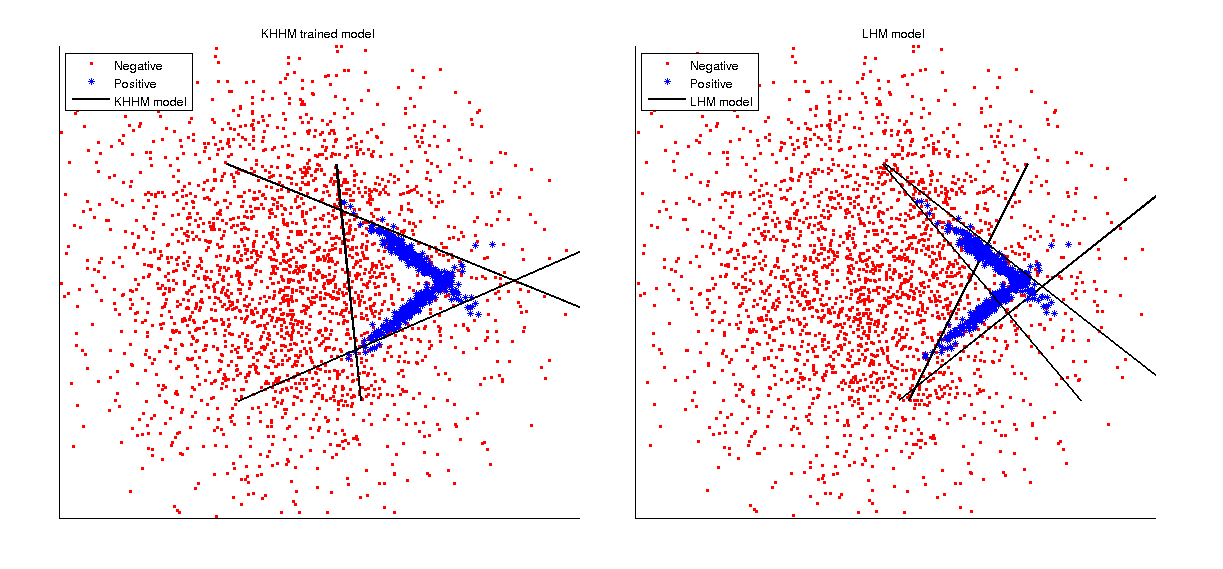
\includegraphics[width=0.8\linewidth]{LHM_vs_KHHM.png}
  \caption{Schematic comparison of KHHM (left) and LHM (right) classifiers on a non-convex positive class. The LHM classifier iteratively discovers a partition of the positive set into convex components and builds KHHM model for each convex component.}\label{fig:khhm_vs_lhm}
  \end{figure}

\subsection{Expected Latent Mixed Risk}
Similarly to K-hyperplane model, the latent mixed risk is also composed of the hinge and background parts. However, we extend the risk  in Eq.~\ref{eq_risk} to contain multiple components $Q^i\triangleq\{x\in R^n| {W^i}^Tx\geq \vec{0}\}$ and a latent variable $\varphi(x)=i$ ($i \in \{1,\ldots,C\}$) which assigns each positive sample $x\in \mathbb{R}^n$  to one of the $C$ components.
\begin{align} \label{eq:lhm_risk}
L_D(\wl;\varphi)=L^{B}_{\mu,\Sigma}(\wl)+L^{H}_D(\wl;\varphi),
\end{align}
The background part of the latent mixed risk bounds the probability of the negative class in all components $Q^i$:
\begin{equation}\label{eq:minimax_expected}
 L^{B}_{\mu,\Sigma}(\wl) = \sum_{i=1}^C {L^B_{\mu,\Sigma}(W^i)}=\sum_{i=1}^C \sup_{z\sim  Z(\mu,\Sigma) }\Pr(z \in Q^i)
\end{equation}
The hinge part of the latent mixed risk aggregates the K-hyperplane hinge risk over $C$ components:
\begin{flalign}\label{eq_expected_hinge_inLHM}
L^H_D(\wl;\varphi)= \mathbb{E}_{(x,y)\in D}\left[\sum_{i=1}^C\ell(W^i;x,y)\mathbbm{1}\left[\varphi(x)=i\right]\right]
\end{flalign}
where $$\ell(W;x,y) = \max_{j\in \{1..K\}}\{\max\{0,\alpha-yw_j^Tx\}\}$$
is the modified K-hyperplane hinge loss (in Eq.~\ref{def_hinge_risk}). We replaced 1 with $\alpha$ to accommodate comparison between different norms of the hyperplanes.



\subsection{Empirical Latent Mixed Risk}
Recall that $S$ is a training sample of size $m$, where $S_2 =\{(x,y)\in S: y = 1\}$, and $S_1=\{(x,y)\in S: y = -1\}$ are the positive and negative training sets correspondingly,  $m_2$ is the size of $S_2$ and $m_1$ be the size of $S_1$. We define the empirical risk over $S$ as follows:
\begin{equation}\label{eq:emp_risk}
L_S^{HB}(\wl,\varphi)=L_{S_2}^H(\wl,\varphi)+L_{S_1}^B(\wl)
\end{equation}
Both parts of the empirical latent mixed risk are aggregated over $C$ latent components. Specifically, the background part of the risk is defined as a sum of background empirical risks of the model's components:
\begin{equation}
%L_{S_1}^M(\wl)=\frac{m_1}{m}\sum_{i=1}^C L_{\hat{\mu},\hat{\Sigma}}^M(W^i)
L_{S_1}^B(\wl)=\sum_{i=1}^C L_{\hat{\mu},\hat{\Sigma}}^B(W^i)
\end{equation}
where $L_{\hat{\mu},\hat{\Sigma}}^B(W^i)={\sup_{Z\in \Omega(\hat{\mu},\hat{\Sigma})} Pr_{z\sim  Z}(z \in Q^i)}$ and $\hat{\mu},\hat{\Sigma}$ are the empirical mean and covariance matrix, estimated from the negative training sample $S_1$.

Let $X^i \triangleq \{x: \varphi(x) = i\}$ define a subset of positive samples. The hinge part of the empirical  risk is defined as the follows:
\begin{equation}
L_{S_2}^H(\wl,\varphi)=\sum_{i=1}^C L_{S_2}^H(W^i)
\end{equation}
where $L_{S_2}^H(W^i)=\sum_{x\in X^i} \ell(W^i,x,1)$.

Using the above notations, we can define a component empirical risk, as
\begin{equation}\label{eq:component_loss}
L^{HB}(W^i)= L_{S_2}^H(W^i)+L_{\hat{\mu},\hat{\Sigma}}^B(W^i)
\end{equation}

Next, we formalize the loss function for a positive sample which we use in the training algorithm in Section~\ref{sec:LHM:training}. Each sample with positive label encounters a loss only in a single latent component, specified by its latent variable $\varphi(x)$. The hinge part of this loss is $\ell(W^i,x,1)$. The background empirical risk of a component $L_{\hat{\mu},\hat{\Sigma}}^M(W^i)$ depends on $\hat{\mu},\hat{\Sigma}$ and $W^i$. $W^i$ depends on the latent assignment of the positive samples. Thus the optimal assignment should minimize also the background part of the risk. We implement this by dividing the empirical risk $L_{\hat{\mu},\hat{\Sigma}}^M(W^i)$ equally among the positive samples with  $\varphi(x)=i$. Hence the sample loss (for positive samples) is defined as follows:
\begin{equation} \label{sample:loss}
L(W^{\varphi(x)};x,1,\varphi(x))=\ell(W^{\varphi(x)},x,1)+
\frac{1}{|S^i|} L_{\hat{\mu},\hat{\Sigma}}^M(W^{\varphi(x)})
\end{equation}
where $|S^i|$ is the  number of samples with $\varphi(x)=i$.

\subsection{LHM Training Algorithm}\label{sec:LHM:training}
The training aims to minimize the empirical risk in Eq. \ref{eq:emp_risk} over the parameters $\wl$ and the hidden variables $\varphi$.  %Similarly to latent SVM~\cite{Yu:2009}, the complexity of the optimal assignment of samples to latent components is exponential.
We propose an iterative algorithm, which reaches fast convergence and shows good results in practice. The algorithm iterates between two steps: First, given an assignment it produces a model $\wl$, second, it updates the latent variables $\varphi(x), \forall (x,y)\in S_2$ to better represent the latent structure of the data.

The \textbf{first} step updates the LHM model $\wl^t$  in iteration $t$ given the latent variables $\varphi$ from iteration $t-1$. Namely, for each hidden component $i=1,...,C$, we find the hyperplanes $W^i$ separating the training samples in $S^i$ from $D_{neg}$ by minimizing the empirical risk in Eq.~\ref{eq:component_loss}. This risk is minimized by the training algorithm proposed in Algorithm 1.

The \textbf{second} step updates the latent variable assignment, given the current $\wl^t$. For each positive sample, it finds the best component w.r.t. the risk in Eq~ \ref{eq:emp_risk}. Specifically, the hinge risk for $x$ is simply $\ell(W^i,x,1)$. The background part of the assignment function for $x\notin Q^i$ should consider the probability that this point adds when it is included in the component $i$ (as shown in Figure~\ref{fig:wx_demo}, left). For $x\in Q^i$, the background part should consider the amount of probability released when the component shrinks as a result of change in the assignment of $x$ (as shown in Figure~\ref{fig:wx_demo}, right). The optimal assignment should take both cases into consideration for all components. To define the assignment function we introduce the following notations.

$W^{def}$ is a \textit{deflated model} derived from $W^i$ by parallel translation of the hyperplane closest to $x$ such that $w_*^Tx+b_*=0$. $W^{inf}$ is an \textit{inflated model} derived from $W^i$ by parallel translation of the hyperplanes for which $w_k^Tx+b_k<0$, until they intersect in $x$, namely, $w_k^Tx+b'_k=0$.  $W^i_x$ is a surrogate model, defined as follows,
$$W^i_x \triangleq  \begin{cases} W^{def} &\mbox{if } x \in Q^i \\
                      W^{inf} &  \mbox{if } x \notin Q^i
        \end{cases}$$ and $Q^i_x\triangleq \{x:{W^i_x}^Tx \geq \vec{0}\}$.
Using the above notations, we define the assignment function as follows,
\begin{equation}\label{eq:argmin}
\varphi(x)= \argmin_{i\in\{1..C\}}{Pr_{z\sim Z}{(z \in Q^i_x)} +\lambda \ell(W^i;x,1)}
\end{equation}
where $\lambda$ is a balancing parameter.
The full training algorithm is summarized in Algorithm~\ref{alg:lhm}.
\begin{figure}
\center
  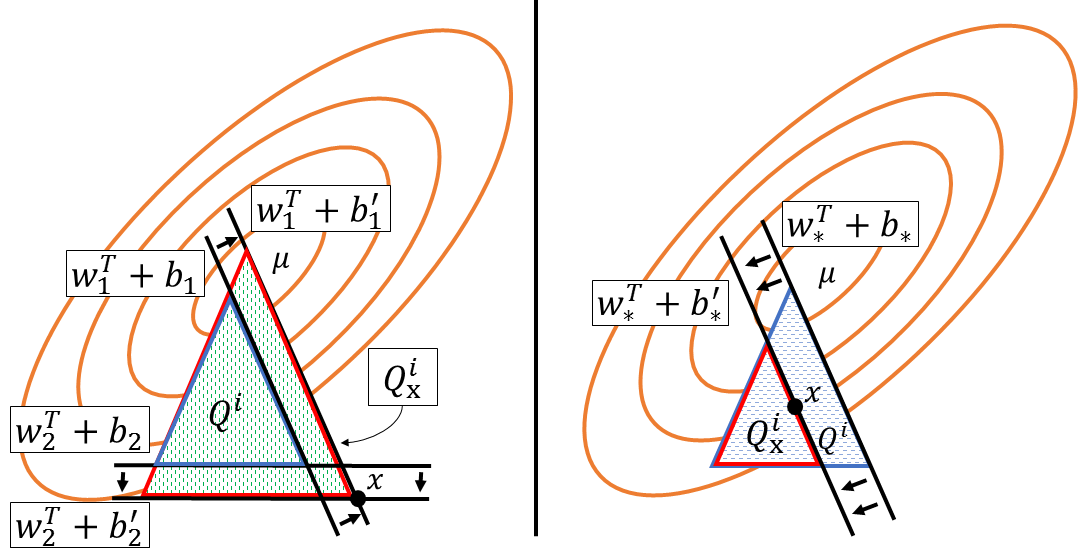
\includegraphics[width=0.5\linewidth]{wx_demo.png}
  \caption{The orange ellipses represent the negative distribution $Z(\hat{\mu},\hat{\Sigma})$, the red triangles corresponds to $Q^i_x$ and  the blue ones to $Q^i$. \textbf{Left}: $w^i_1, w^i_2$ are moved to pass through $x$, causing the probability $Q^i$ to increase. \textbf{Right}:$w^i_*$ is moved to pass through $x$, causing the probability $Q^i$ to decrease.}
  \label{fig:wx_demo}
\end{figure}
\begin{algorithm}
\caption{LHM Training. $T$ is the threshold on the empirical risk change.}
\label{alg:lhm}
\begin{algorithmic}
%\INPUT{$C$, $K$, $S_1$, $S_2$,$T$}
\STATE\textbf{Input: }$C$, $K$, $S_1$, $S_2$,$T$
%\OUTPUT{$\wl,\varphi$}
%\STATE\textbf{Output: }$\wl,\varphi$
\STATE \textbf{Initialization:} \\\hspace{0.5cm}
$t \gets 1$ \\\hspace{0.5cm}
$L(\wl^{t=0};\varphi^{t=0}) \gets \infty$ \\\hspace{0.5cm}
$\varphi^t \gets Init(S_2,C)$  
\STATE
\STATE \textbf{Training:} \\\hspace{0.5cm}
\textbf{while }$L(\wl^t;\varphi^t) - L(\wl^{t-1};\varphi^{t-1}) \ge T$ \textbf{do}\\\hspace{1cm}
\COMMENT{Model Step}\\\hspace{1cm}
\textbf{for i=1 to C} \textbf{do}\\\hspace{1.5cm}
$W^{i,t}=$\emph{KHHM-training}($S_1$,$X^i$) \COMMENT{in Algorithm 1}\\\hspace{1cm}
\textbf{end for}\\\hspace{1cm}
\COMMENT{Assignment Step}\\\hspace{1cm}
\textbf{for{$(x,y)\in S_2$}}\\\hspace{1.5cm}
$\varphi^{t+1}(x)$ as defined in Eq.~\ref{eq:argmin}\\\hspace{1cm}
\textbf{end for}\\\hspace{1cm}
$ t \gets t+1 $ \\\hspace{0.5cm}
\textbf{end while}
%\WHILE{$L(\wl^t;\varphi^t) - L(\wl^{t-1};\varphi^{t-1}) \ge T$}
%  \STATE\COMMENT{Model Step}
%  \FOR{i=1 to C}
%     \STATE $W^{i,t}=$\emph{KHHM-training}($S_1$,$X^i$) \COMMENT{in Algorithm 1}
%  \ENDFOR
%  \STATE\COMMENT{Assignment Step}
%  \FOR{$(x,y)\in S_2$}
%    \STATE $\varphi^{t+1}(x)$ as defined in Eq.~\ref{eq:argmin}
%  \ENDFOR
%  \STATE $ t \gets t+1 $
%\ENDWHILE
\STATE\textbf{Output: }$\wl,\varphi$
\end{algorithmic}
\end{algorithm}

\begin{lemma}
Algorithm~\ref{alg:lhm} %minimizes
reduces the empirical risk $L_S^{HB}(\wl;\varphi)$ in each iteration.
\end{lemma}

\begin{proof}
Since latent mixed risk is a sum of risks over the latent components (Eq.~\ref{eq:emp_risk}), it is minimized by minimizing the empirical risk of each component. In step (5) of the Algorithm~\ref{alg:lhm}, we train $W^{i,t}$ model for each latent component $i=1,...,C$  using Algorithm 1  (Section~\ref{KHHM_Alg}). It is easy to see that $L_S^{HB}(W^i) = L^{HB}_S(W)$ (in Eq.~\ref{eq_emp_risk}), thus step (5) of the Algorithm~\ref{alg:lhm} minimizes the component's risk in Eq.~\ref{eq:component_loss}.

It is now left to show that the assignment $\varphi^t$ in iteration $t$, will cause the reduction in the empirical risk in iteration $t+1$. Since the empirical risk is aggregated over positive samples, it is enough to prove the claim for a single sample. We consider two cases:

\noindent\textbf{1.} The  assignment of sample $x$ does not change, formally $\varphi^{t}(x)=\varphi^{t+1}(x)$. \newline
\noindent In this case $L(\wl^{t+1};\varphi^{t+1}(x))$ will only be affected by the $W^{i,t+1}$ training, thus
\begin{equation}
L\left(\wl^t;\varphi^t(x)\right)\ge
L\left(\wl^{t+1};\varphi^{t+1}(x)\right)
\end{equation}

\noindent\textbf{2.} The assignment of sample $x$  is changed. Formally, in iteration $t$: $\varphi^{t}(x)=i$ and in iteration $t+1$, exists $j \ne i$,  such that
\begin{equation}
\varphi^{t+1}(x)=j=
\argmin_{k\in\{1..C\}} {L^B_{S_1} \left(W^{k,t}_x\right)+ \lambda L^H_{S_2}\left(W^{k,t};x\right)}.
\end{equation}
Since $x \in Q^i$, reassigning it to a different component will cause  the $Pr_{z\sim Z}(z \in Q^i_x)$ to decrease (or stay the same), thus
\begin{equation}
L^B_{S_1}(W^{i,t}_x) - L^B_{S_2}(W^{i,t}) \le 0.
\end{equation}
Hence, the sample loss in component $i$ is larger than the sample loss in the deflated component:
\begin{equation}\label{eq:9}
L\left(W^{i,t};x\right) \geq L^B_{S_1}\left(W^{i,t}_x\right) + \lambda L^H_{S_2}\left(W^{i,t};x\right).
\end{equation}
At the same time, $j$ is the optimal assignment, thus
\begin{equation}\label{eq:10}
L^B_{S_1}\left(W^{i,t}_x\right) + \lambda L^H_{S_2}\left(W^{i,t};x\right) \ge L^B_{S_1}\left(W^{j,t}_x\right) + \lambda L^H_{S_2}\left(W^{j,t};x\right).
\end{equation}
Since $W^{j,t}_x$ is a naive inflation of $W^{j,t}$ to include $x$, the solution  $W^{j,t+1}$, provided by KHHM training, would have lower (or same) empirical risk, thus
\begin{equation}\label{eq:11}
L^B_{S_1}\left(W^{j,t}_x\right)\geq L^B_{S_1}(W^{j,t+1}).
\end{equation}
In iteration $t+1$, $x$ is included in $X^j$ for training  the $j$'th latent component, consequently
\begin{equation}\label{eq:12}
L^H_{S_2}\left(W^{j,t};x\right)\geq L^H_{S_2}(W^{j,t+1};x).
\end{equation}
(as we assume that $x\in X^j$ leads to $x\in Q^{j,t+1}$).
Finally, by combining the inequalities in Eq.~\ref{eq:9}--\ref{eq:12}, we obtain:
\begin{equation}
L\left(W^{i,t};x\right) \geq L\left(W^{j,t+1};x\right).
\end{equation}
\end{proof}
\subsection{Generalization Bound for LHM Model with Fixed Assignment}
For a fixed $\varphi(x), \forall (x,y)\in S_2$, we can derive a uniform generalization bound for the union of the K-hyperplane models. Similarly to KHHM model (in Section~\ref{sec:khhm_bond}), we derive the uniform generalization bounds separately for the positive and negative classes.  We start with the positive class, for which we use the hinge part of the latent mixed risk.
%hinge part
\begin{theorem}
Let $\varphi^*$ denote a fixed assignment of the positive training samples to components.
Let  $L^H_D(\wl;\varphi^*)= \mathbb{E}_{(x,y)\in D}\left[\sum_{i=1}^C\ell(W^i;x,y)\mathbbm{1}\left[\varphi^*(x)=i\right]\right]$ be the expected risk, and let $L_{S_2}^H(\wl,\varphi^*)=\sum_{i=1}^C L_{S_2}^H(W^i)$ be the empirical risk over a positive label training sample of size $m_2$ for a fixed assignment $\varphi^*$  of the positive samples to $C$ components. Then, for any $\delta \in (0,1]$ with probability at least $1-\delta$ over the i.i.d. sample of size $m_2$ it holds simultaneously for all  $\|w_i\|\le 1$ ($i=1,...,C\cdot K$) that whenever $\|x\|  \le 1$:

$$L^H_D(\wl;\varphi^*) \le  L_{S_2}^H(\wl,\varphi^*) + \sqrt{\frac{\log 1/\delta}{2m_2}}L_{S_2}^H(\wl,\varphi^*) +\max_{i\in \{1,...,C\}}\left({\frac{2K}{\sqrt{m^i}} + 8K\sqrt{\frac{2 \log(2/\delta)}{m_2}}}\right)$$

\end{theorem}
\begin{proof}
Let $p_i = E_{(x,1) \sim D} \Big[\mathbbm{1}[\varphi^*(x)=i] \Big]$, and let $\frac{m_i}{m^+}$ be its estimated mean. Then,
\begin{flalign}\label{eq:21}
\nonumber &L^H_D(\wl;\varphi^*) -  L_{S_2}^H(\wl,\varphi^*) = \sum_{i=1}^C{\left(p_iL_D^H(W^i)-\frac{m_i}{m_2}L^H_{S^+}(W^i) \right)}\\
&=\sum_{i=1}^C \left[p_i\left(L_D^H(W^i)-L^H_{S_2}(W^i)\right)\right]+  \sum_{i=1}^C\left[(p_i-\frac{m_i}{m^+})L^H_{S_2}(W^i)\right]&&
\end{flalign}
We can bound the discrepancy between the expected and empirical risks in a component using Theorem~\ref{th_10}. Hence, the first term in Eq.~\ref{eq:21} is upper bounded by $\max_{i\in\{1,...,C\}}\left({\frac{2K}{\sqrt{m^i}} + 8K\sqrt{\frac{2 \log(2/\delta)}{m_2}}}\right)$. We can upper bound $(p_i-\frac{m_i}{m_2})$ using the Hoeffding inequality.  Rearranging the terms and noting that $\sum_{i=1}^C L^H_{S_2}(W^i)= L_{S_2}^H(\wl,\varphi^*)$ conclude the proof.
\end{proof}
We formulate the uniform generalization bound for the negative class below.
%minimax part
\begin{theorem}
Suppose that $D$ is a distribution over $X \times Y$ such that $Y = \{-1,+1\}$ and $X = \{x: \|x\| \le G\}$. Let $L_{\mu,\Sigma}^{B}(\wl;\varphi^*)$ be the background risk over the negative labels, where $\mu, \Sigma$ are the mean and covariance of the marginal distribution of $x$ over the negative labels and the positive labeled samples have a fixed assignment $\varphi^*$. Consider a training sample $S$ of size $m$, $m_1$ of which have negative label and let $$L_{\hat \mu,\hat \Sigma}^{B}(\wl;\varphi^*) = \sum_{i=1}^C L_{\hat \mu,\hat \Sigma}^{B}(W^i)$$  be the empirical background risk over the negative labels ($\hat \mu, \hat \Sigma$ are the empirical mean and covariance estimation of $D_{neg}$). %the marginal distribution of $x$ over the negative training labels. Then, for any $\delta \in (0,1]$ with probability at least $1-3\delta$ over the i.i.d. sample of size  $m>\log(1/\delta)$, the following holds uniformly for all $W$:
With probability at least $1-3\delta$ over $m_1$ the i.i.d. samples from $D_{neg}$ the following holds uniformly for all $W$ including $C$ components, each with $K$ independent hyperplanes:

 $$L_{\mu,\Sigma}^{B}(\wl;\varphi^*) \le L_{\hat \mu,\hat \Sigma}^{B}(\wl;\varphi^*) + C\Big(\frac{2G^2 }{\alpha} + \frac{6G^4}{\alpha^2} \Big) \sqrt{\frac{32(\log(1/\delta) + 1/4)}{m_1}}.$$

%$$L_{\mu,\Sigma}^{M}(\wl;\varphi^*) = \ L_{\hat \mu,\hat \Sigma}^{M}(\wl;\varphi^*)+ C\left(\sqrt{\frac{log(1/\delta)}{2m}}+r \sqrt{\frac{32(\log(1/\delta) + 1/4)}{m^-}}\right),$$
%where
%$r = 2/\alpha + 1/\alpha^2+1$ and $\alpha$ is the minimal eigenvalue of $\Sigma, \hat \Sigma$.
\end{theorem}
The proof is straightforward as the assignment $\varphi^*$ does not affect negative samples, and thus the bound is a simple summation of bounds for each component which is derived using Theorem~\ref{theorem:minimax1}.


\section{Mapping LHM Classifier to a Neural Network}
Deep Neural Networks and Convolutional Neural Networks (CNN) in particular have shown impressive results in a variety of domains, including images, speech, text, etc. CNN enables learning very good features for these domains, but requires a lot of labeled training samples. One way to reduce the number of examples needed for training of a specific classification task is to pre-train a CNN on a different classification problem in a similar domain and then change the last layer of the CNN to fit the target classification problem and fine-tune the network on a smaller training set associated with the target problem. This approach is referred to as transfer learning. %It works, because the lower layers of the CNN learn good features using the larger set, while training the upper layer requires significantly less training data.

%We show that using LHM-NN in the transfer learning settings has significant benefits compared to NN (standard settings), in both classification accuracy and training efficiency. The improved accuracy stems from the ability of LHM model to learn from unlabeled data. The fast convergence of the LHM-NN (just a handful of epochs) is due to a very good initialization of the upper layers with class specific LHM classifiers. Note that class specific LHM models can be trained in parallel.

When the target classification problem is less similar to that used to train CNN features, the classification accuracy of the fine-tuned network could be quite poor. This is because the high-level representation of the original and the target networks are different. One way to approach this problem is by employing a non-linear classifier, such as LHM classifier, on  CNN features. In order to fine-tune the feature layers with the LHM classifier, we need to combine them in a single architecture. To this end we  propose to map LHM Classifier to a Neural Network and stack it on top of the pre-trained convolutional layers. This enables end-to-end training of feature extraction and classifier.
%and 2) LHM generalization to multi-class that enables using a smaller number of labeled training samples than NN.
As we show below, mapping of LHM classifier to NN also allows extending it to multi-class problems.

\subsection{Binary NN}\label{sec:binary_nn}
\begin{figure}
\center
  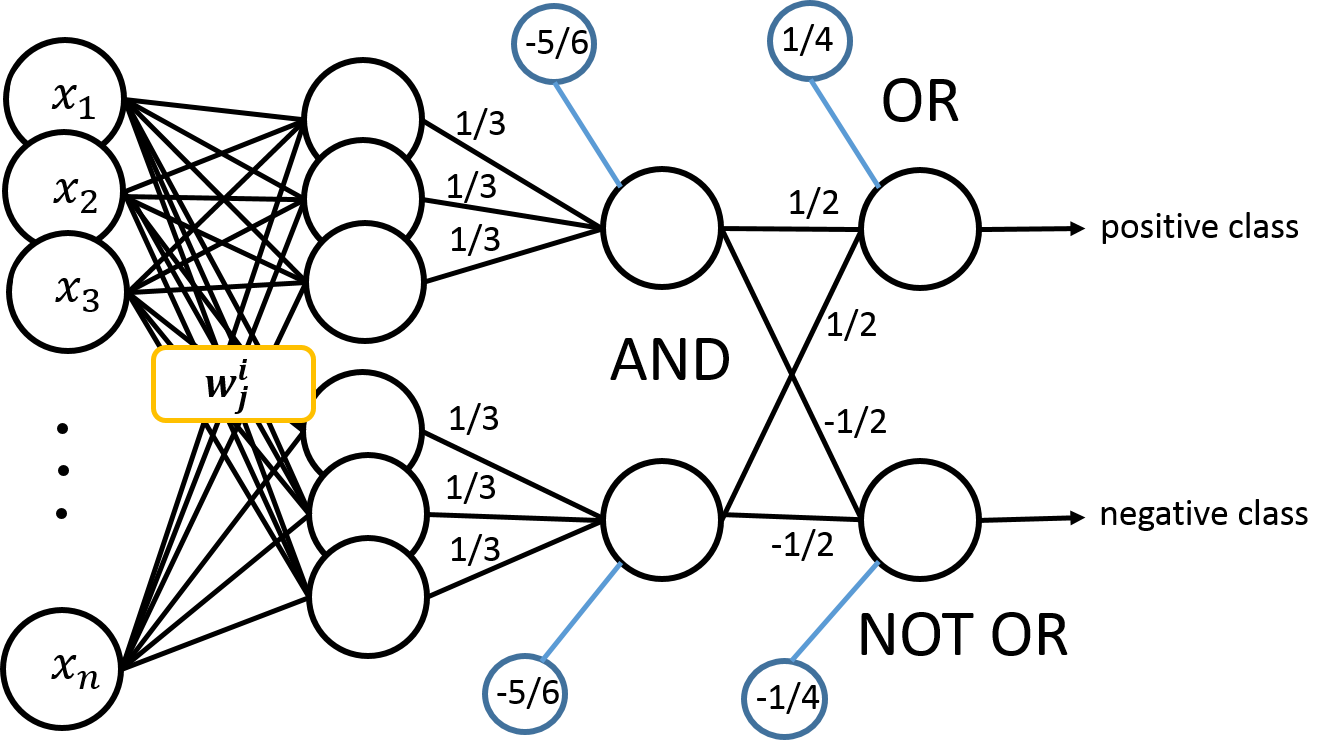
\includegraphics[width=0.7\linewidth]{LHM_NN_arch.png}
  \caption{An example of NN equivalent to LHM for two components and three hyperplanes in each.} %The input vector $x$ is projected on six hyperplanes from two latent clusters. For each latent cluster, the three projection are summed and is activated only if all are positive. On the third layer the latent clusters are summed again and activate the output if at least one of the latent clusters was activated.}
  \label{fig:LHM_NN}
\end{figure}
 A union of the intersections of positive half spaces can be implemented by a NN with three hidden layers. The first fully connected hidden layer has $K\times C$ neurons with a sigmoid activation, where $K$ is the number of hyperplanes in an intersection and $C$ is the number of components. The second hidden layer has $C$ nodes with a sigmoid activation, connected only to the neurons associated with hyperplanes forming the corresponding intersection. The weights on these connections and the biases are fixed and mimic \textbf{AND} operation, namely, all weights of this layer are equal to $1/K$ and the biases are equal to $-1+1/(2K)$.  The last hidden layer has two neurons, which are fully connected to the previous layer with the fixed weights and biases, one of which mimics \textbf{OR} operation, and the other  \textbf{NOT OR}. Namely, the neuron, corresponding to OR has  weights equal to $1/C$   and the bias of $-1/(2C)$. The neuron corresponding to NOT OR  has weights equal to $-1/C$ and the bias of $1/(2C)$.  The network has two outputs, one for the positive class (with label 1) and one for the negative class (with label 0). An example of such network for $C=2$ and $K=3$ is depicted in Figure~\ref{fig:LHM_NN}.

\subsection{Multi-Class NN}\label{sec:mc_nn}
For a multi-class setting, we suggest to train LHM model for each class using an additional unlabeled data for estimating the statistics of the negative class. We then map these models to a multi-class NN with the following architecture. The first hidden layer  is a fully connected layer with $C\times K$ neurons per class, $C\times K\times G$ neurons in total, where $G$ is the number of classes. These are  equivalent to  $C\times K\times G$ hyperplanes in the LHM model. For each hidden component, all hyperplanes in the intersection are connected to their corresponding node in the \textbf{AND} layer (as detailed in Section~\ref{sec:binary_nn}). The \textbf{AND} layer comprises $C\times G$ neurons. The next layer is a fully connected layer, comprising $G$ nodes. The weights on the connections to the $C$ components of the corresponding class are initialized with 1's, and the weights on the remaining connections are initialized with very small values from a Gaussian distribution.  The network has $G$ outputs and is trained using the cross-entropy loss.

To provide an end-to-end training, one can consider stacking the feature extraction layers of CNN (up to fully connected layers) with one of the above networks.


\section{Experiments}
We start by evaluating the simple K-hyperplane model (Section~\ref{sec:exp:KHHM}) and then move to a more general LHM model (Section~\ref{sec:exp:LHM}). Both models are tested on synthetic and real data. Then we show how the hinge-minimax training can be combined with a CNN (Section~\ref{sec:cifar_ex}) for approaching problems that require more powerful features but do not have large enough data to train a deep model from scratch. We demonstrate this for both binary and multi-class settings.

\subsection{K-Hyperplane Hinge-Minimax Classifier}\label{sec:exp:KHHM}
To test the proposed  KHHM classifier,
we ran experiments in three different scenarios: synthetic 2D data, letter recognition,
and large scale scene classification.

During classification, the $K$-hyperplane classifier incurs
only $K$ times the computational complexity of
a linear classifier (just $K$ inner products), hence its ``natural
competitors'' are linear classifiers, and we choose linear SVM for the benchmark.
\begin{figure*}
\center
\begin{tabular}{ccc}
 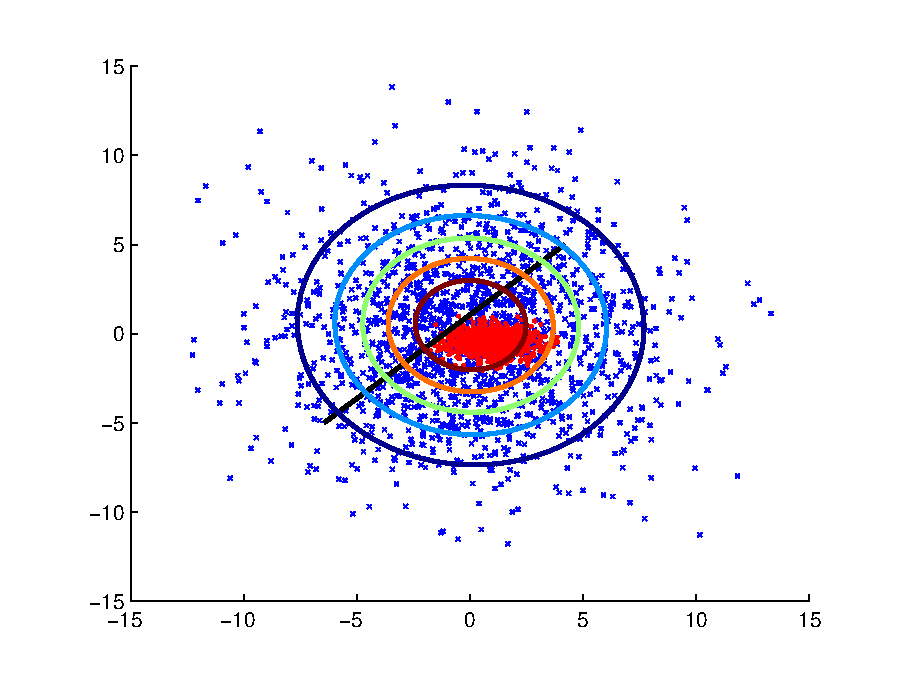
\includegraphics[width=2in]{ex_5_1.eps}
&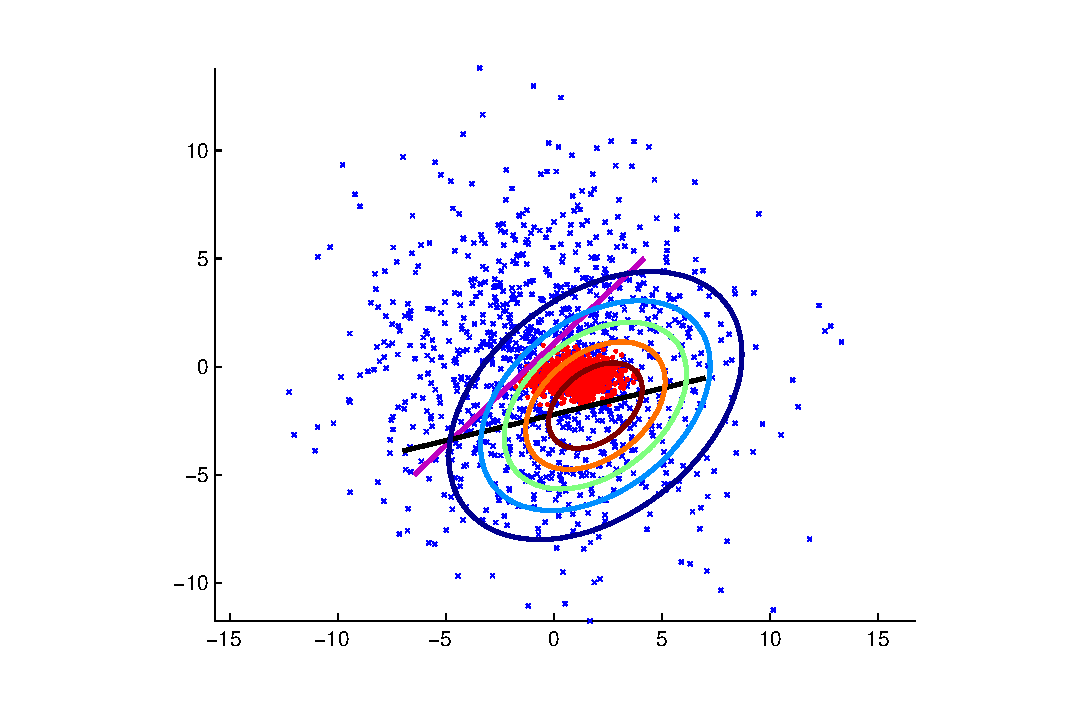
\includegraphics[width=2in]{ex_5_2.eps}
& 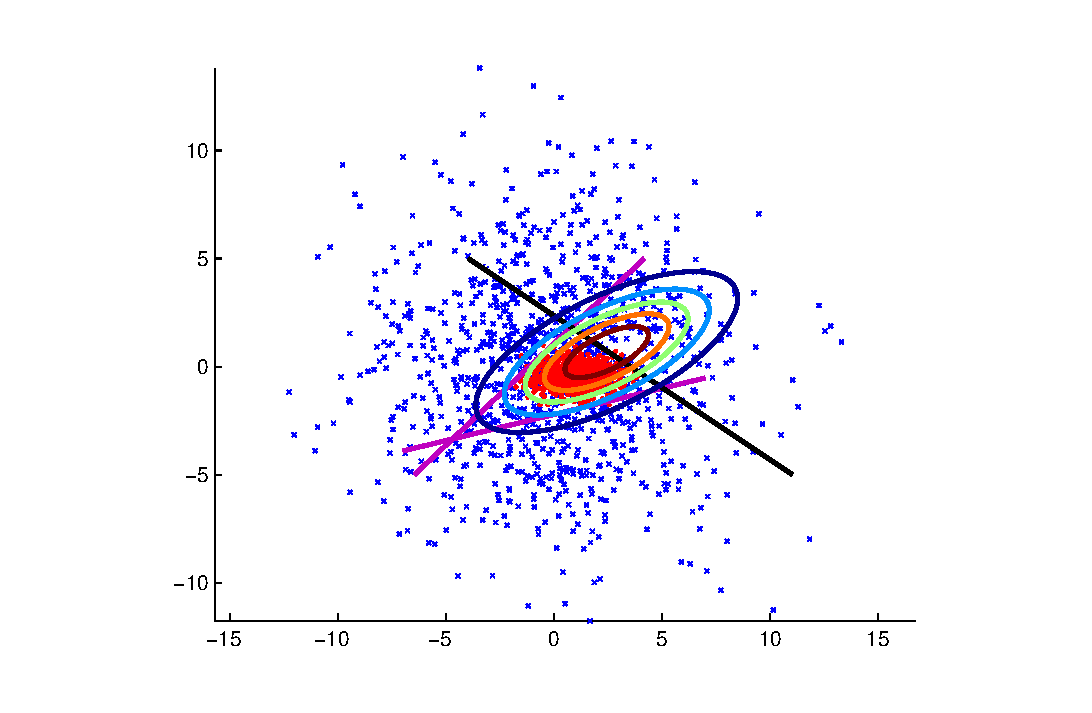
\includegraphics[width=2in]{ex_5_3.eps} \\
  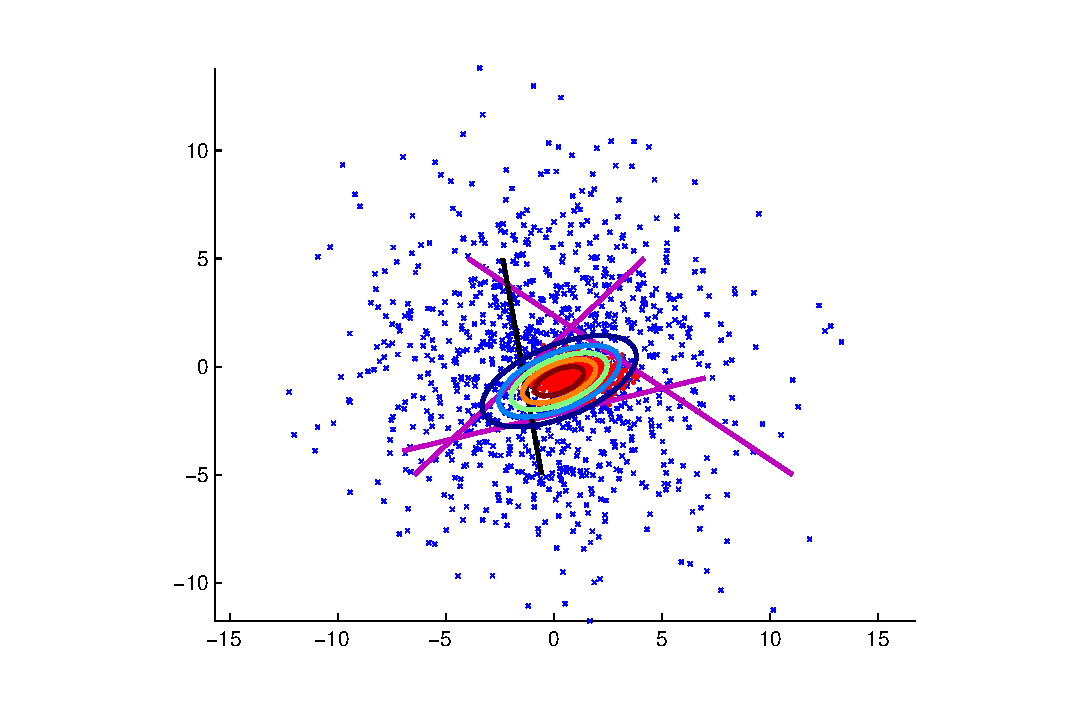
\includegraphics[width=2in]{ex_5_4.eps}
& 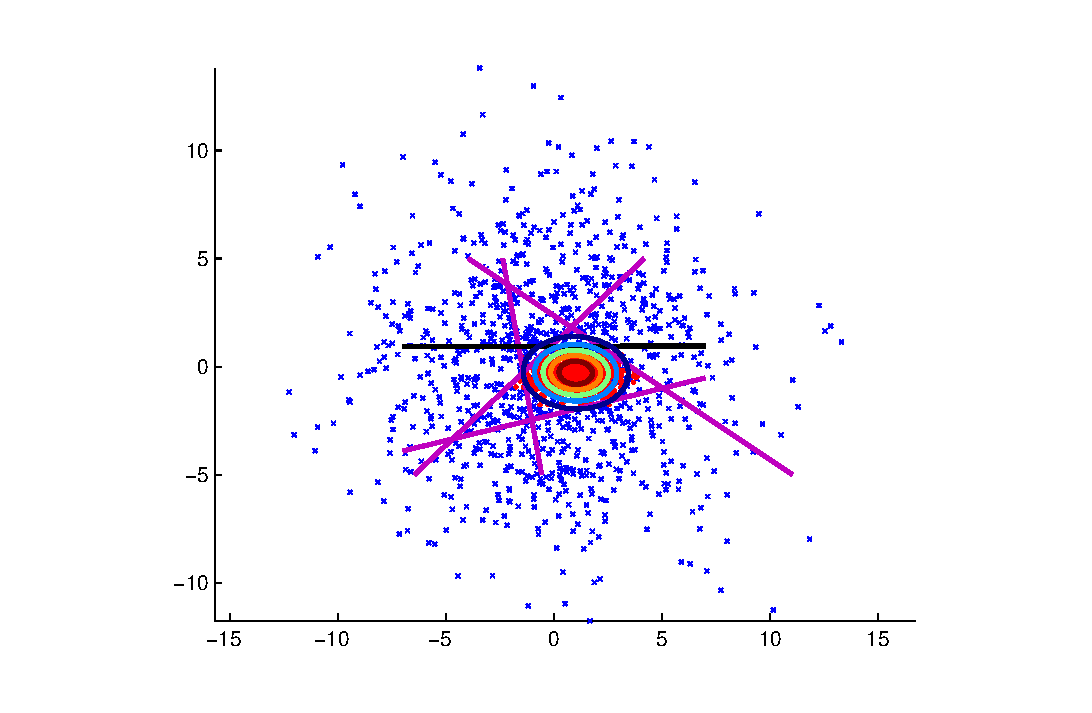
\includegraphics[width=2in]{ex_5_5.eps}
& 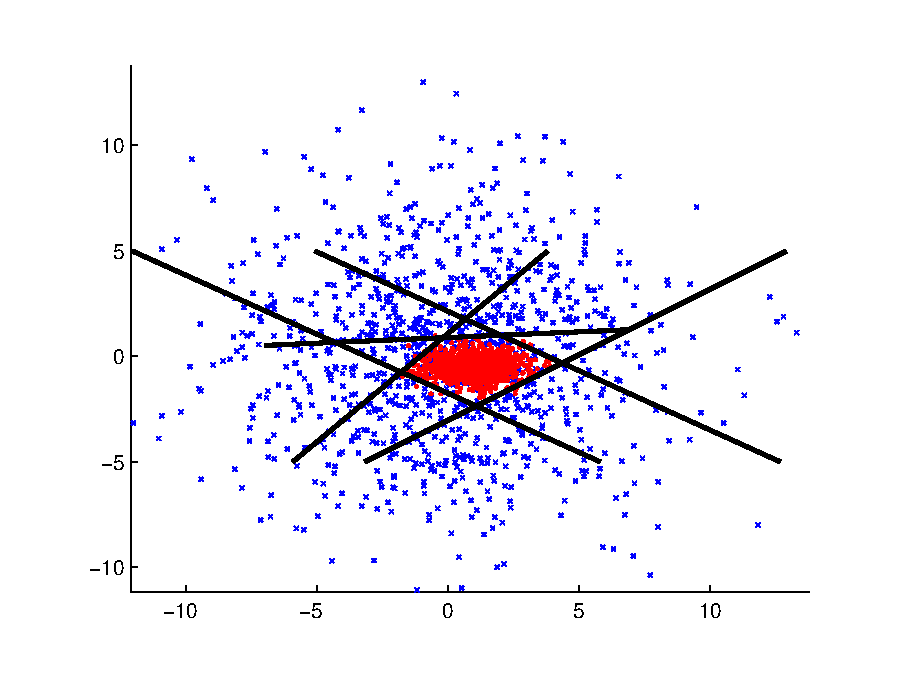
\includegraphics[width=2in]{ex_5_final.eps}
\end{tabular}
\caption {Illustration of KHHM classifier construction on a toy example.The first 5 figures show the greedy initial step. The last figure shows the final classifier after 25 iterations. The contour lines show the covariance matrix of the negative distribution inside the intersection of hyperplane, which is used to find the optimal hyperplane, depicted in black.}
\label{fig_toy_ex}
\end{figure*}
We have also compared the hinge-minimax classifiers to kernel SVM and
ensemble-based methods, which incur far longer running
times (this is especially true for kernel SVM). The classification rates of the hinge-minimax classifier in all our experiments were comparable to ensemble classifiers which required 100-170 basic classifiers in order to reach similar performance. In experiments with high-dimensional data, the KHHM  classifiers preformed as well as kernel SVM.

The SVM classifiers were trained using C-SVC
in LIBSVM \footnote{$http://www.csie.ntu.edu.tw/
cjlin/libsvm/$}. We used the CVX optimization package
\footnote{$http://cvxr.com/cvx/download/$} to find a single hyperplane in Algorithm 1. The ensemble classifiers were trained using the
Matlab Statistic toolbox.

\subsubsection{Synthetic Data Example}
We construct the KHHM classifier for  2D data to illustrate Algorithm 1. We samples 5000 data points from two highly overlapping Gaussians (see Figure \ref{fig_toy_ex}) with varying ratio of positive (shown in red) and negative (shown in blue) examples. Each class was equally partitioned into training, validation, and test sets. We estimated the mean and covariance from the training data and tuned the parameters (C and $\gamma$) and the bias using the validation set. Table \ref{TAB:AUC} shows the AUC for the different ratios of positive and negative examples using an intersection of 5 hyperplanes. These results demonstrate the robustness of the algorithm to imbalanced sets.

\begin{table}[h!]
\center
\scalebox{0.9}{
  \begin{tabular}{|c|c|c|c|c|c|c|}
  \hline
  Positive &0.01 &0.1&0.2&0.3&0.4&0.5\\
  fraction& & & & & & \\
  \hline
  AUC&94.68& 94.91& 95.07 & 94.96 & 94.89 & 95.83\\
\hline
\end{tabular}}
\caption{AUC for different size partitions of positive and negative classes}\label{TAB:AUC}
\end{table}

The first five plots in Figure \ref{fig_toy_ex} show the result of the initial greedy step for the first, second, third, forth, and fifth hyperplanes respectively. The contour lines in Figure \ref{fig_toy_ex} illustrate the covariance of the negative distribution inside the intersection, which is used to find the optimal separation hyperplane, depicted in black. The last plot in Figure \ref{fig_toy_ex} shows the final classifier after 25 iterations. It illustrates that the approximation algorithm succeeds in separating the positive set from the background, and that the refinement iterations improve the separation boundary.

\subsubsection{Letter Recognition}
The following tests were performed  on a data set of letters  from
the UCI Machine Learning
Repository (\cite{UCIrep}), which includes 16-dimensional feature
vectors for the 26
letters in the English alphabet. The letter images were based on 20
different fonts and each letter within these 20 fonts was randomly
distorted to produce 20,000 samples. For each letter, we used
100 samples for training, 250 for validation, and the
rest for test (about 400 samples per letter). The parameters of all methods have
been chosen using the validation set. Since the test set includes 25 times
more negatives than positives, which leads to about 96\%
classification rate by just classifying all inputs as negative,
we used EER as a more faithful measure of performance.
\begin{table}[h!]
\center
\begin{tabular}{|c|c|c|}
\hline
  % after \\: \hline or \cline{col1-col2} \cline{col3-col4} ...
  Method & Classification  & Classification \\
  &rate at EER& time\\
  \hline
  KHHM $K=1$  & 89.32 &  5.6e-07 \\
  KHHM $K=2$  & 92.98 &  1.4e-06\\
  KHHM $K=3$  & 93.93 &  1.5e-06\\
  KHHM $K=4$  & 94.48 &  1.7e-06\\
  Linear SVM           & 84.87 &  4.6e-07\\
  RBF kernel SVM       &96.47  &  1.7e-03\\
  AdaBoost             & 92.26 &  1.0e-03\\
\hline
\end{tabular}
\caption{Letter experiments. $K$ corresponds to the number of hyperplanes used in the hinge-minimax classifier. The times are in sec.
AdaBoost uses 100 decision trees.}\label{letters}
\end{table}
 Table \ref{letters} shows the classification rate at EER , averaged over 26
letters, and the average classification times of the
tested classifiers.

The KHHM classifiers improve over the linear SVM for all $K$, and for $K>1$
outperforms Adaboost with much shorter classification time. For this data set, kernel SVM outperform all methods. However, the KHHM classifier with $K=4$ comes fairly close to the performance of the kernel SVM, while its classification time is three magnitudes faster.
%
%


\subsubsection {Large Scale Scene Recognition}
\label{sub:SUN}

In this test we used 397 scene categories of the SUN data base, which have at least 100 images per  category (\cite{SUN}). We represent the images as BOW of dense HOG features with 300 words. We downloaded the features from the SUN web page\footnote{$http://vision.cs.princeton.edu/projects/2010/SUN/$}, containing spatial pyramid of BOWs, and used the bottom layer (the details of the feature extraction can be found in \cite{SUN}).  The data is divided into 50 training and 50 test images in 10 folds. Training one-against-all classifiers for 397 categories with 50 training samples per category uses very unbalanced training sets. Thus we defined different weights for positive and negative samples in SVM training and we used RUSBoost (\cite{RUSboost}) as an ensemble method (it is designed for skewed data and performed significantly better than AdaBoost on this data set). Note that the KHHM classifier naturally handles imbalanced sets. KHHM classifier with more than two hyperplanes didn't improve the performance. Table \ref{SUN300} shows the average AUC of the tested methods and their running times.
\begin{table}
\label{SUN300}
\center
\begin{tabular}{|c|c|c|}
  \hline
  % after \\: \hline or \cline{col1-col2} \cline{col3-col4} ...
  Method & AUC  & classification \\
  & &time\\
   \hline
  KHHM $K=1$  & 88.89 & 9.8e-05\\
  KHHM $K=2$ & 90.99 & 1.34e-04  \\
  Linear SVM             & 88.20 & 8.6e-05  \\
  RBF kernel SVM         & 90.77 & 23.97\\
  RUSBoost               &90.76  &0.08  \\
  \hline
\end{tabular}
\caption{Scene classification with 300 dim. features. The classification time of RBF kernel SVM is very high, since it chooses about 15,000 SVs from 19850 training examples. The RUSBoost uses 100 decision trees.}
\end{table}
\begin{figure}
\center
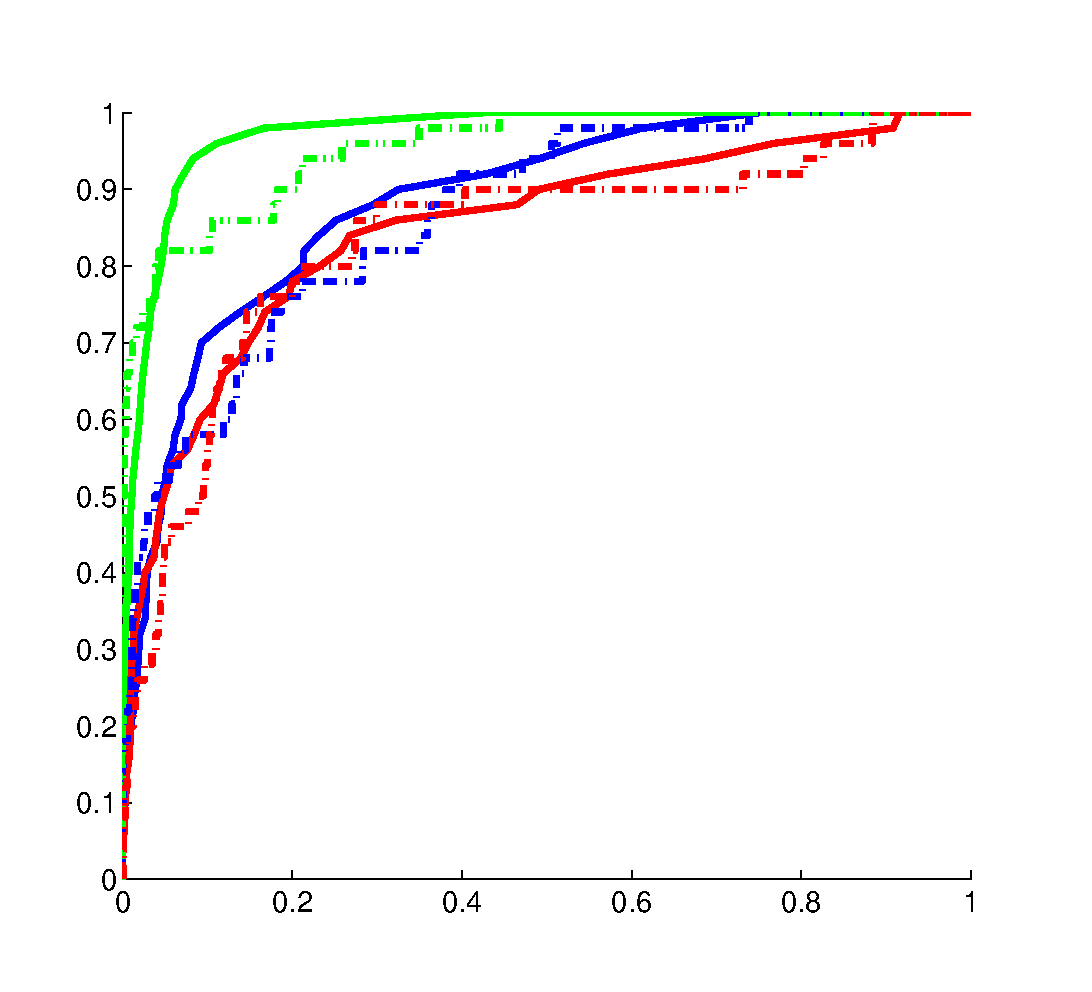
\includegraphics[width=3in]{combFullD.eps}
\caption {ROCs of the first three categories of the SUN data set, represented by  a spatial pyramid of BOWs, obtained from dense HOG. The solid lines correspond to the hinge-minimax classifier, dotted lines correspond to the histogram intersection kernel SVM.}
\label{SUN_fullD}
\end{figure}

Using a pyramid of BOWs with the histogram intersection kernel improves
over the RBF kernel applied to the bottom layer of the pyramid,
but then the dimension of the feature vector increases to 6300. The AUC  of the KHHM classifier with $K=2$ is 92.99\% and of histogram kernel is 92.85\%. Figure \ref{SUN_fullD} shows the ROCs of the first three categories produced by the KHHM classifier and the histogram intersection kernel SVM classifiers.
%%%%%%%%%%%%%%%%%%%%%%%%%%%%%%%%%%%%%%%%%%%%%%%%%%%%%%%%%%%%%%%%%%%%%%%%%%

\subsection{Latent Hinge Minimax Classifier}\label{sec:exp:LHM}
We first show a 2D toy example (Section~\ref{sec:synthetic_ex}) to illustrate the ability of the LHM classifier to discover the hidden components in the positive class and to separate each of them from the negative class using a K-hyperplane model.

Then, we compare LHM model to alternative ensembles of hyperplanes (in shallow architectures) on the PASCAL-VOC 2007 dataset (\cite{Everingham10}) (Section~\ref{sec:voc_ex}), and show its advantage over those methods and its robustness to the choice of the number of latent components.

\begin{figure}[t]
\center
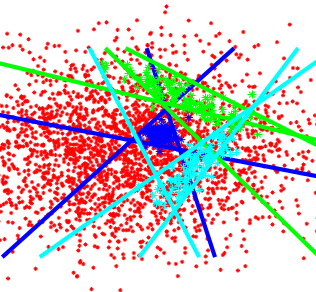
\includegraphics[width=1.6in]{MW_bad_clustering_new.png}\hspace{0.4cm}
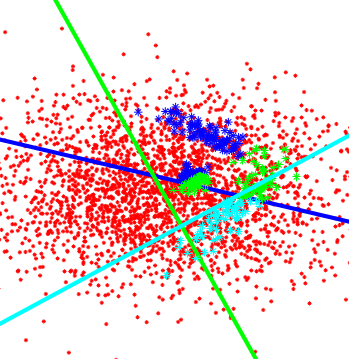
\includegraphics[width=1.6in]{LDA_OR_bad_clustering.png}
\caption{A qualitative comparison of the latent hinge minimax classifier (on the left) to the union of LDA classifiers (on the right).}
\label{LDAvsLHM_toy}
\end{figure}

\begin{figure*}[h]
\center
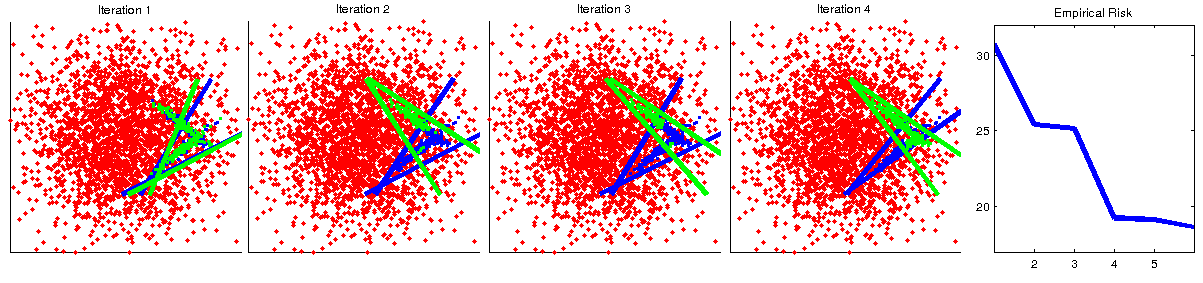
\includegraphics[width=\linewidth]{demo2.png}
\caption{First four iterations of the LHM training on toy example and the corresponding loss convergence. }
\label{fig:2d_example2}
\end{figure*}
\subsubsection{Synthetic Data}\label{sec:synthetic_ex}
A simpler alternative to the LHM model is a two-step algorithm which first finds the structure of the target class by applying some kind of unsupervised learning (e.g, k-means clustering) and then builds a model for each component. Such a simple approach was employed in~\cite{Deva} with LDA classifier (\cite{LDA}) trained per cluster. Unless the clusters are very small\footnote{as in time consuming exemplar-based approach(\cite{eSVM})}, it relies heavily on the results of the clustering. If an initial clustering is incorrect (as in Figure \ref{LDAvsLHM_toy}, right), LDA (or any other convex classifier) cannot separate the resulting components from the background without including many false positives.  The LHM  training finds the underlying structure of the data and the model iteratively, improving both (Figure~\ref{LDAvsLHM_toy}, left). Furthermore, LHM is quite robust to the initial assignment. Figure~\ref{fig:2d_example2} shows a few iterations and the corresponding loss convergence when the  initial assignment of the positive samples to components is chosen at random. Note the LHM training discovers the underlying structure in a 3-4 iterations.

\begin{figure}[t]
\center
  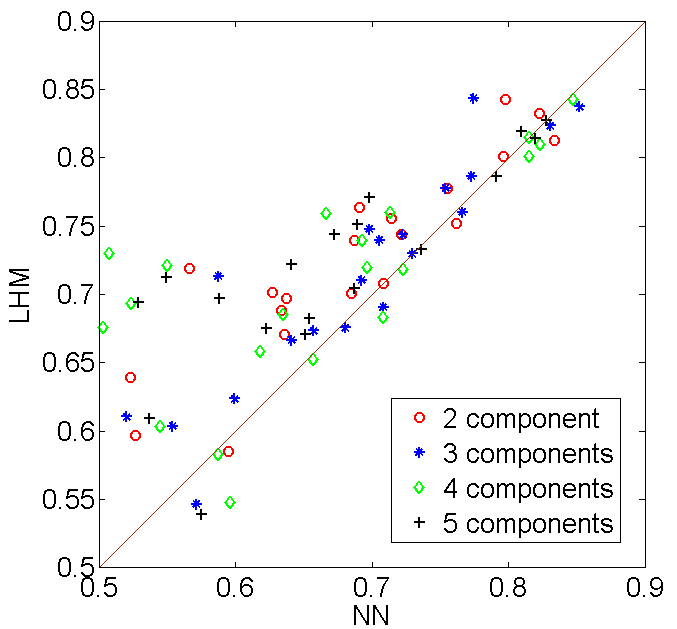
\includegraphics[width=0.5\linewidth]{VOC_LHMvsNN.png}
  \caption{Comparison of the LHM classifier to the equivalent NN for a varying number of hidden components (from 2 to 5) on PASCAL VOC 2007. %Comparison of the LHM classifier (the y-axis) to the equivalent NN (x-axis) for a varying number of assumed hidden components (from 2 to 5) on PASCAL VOC 2007.
  The points above the diagonal line show the advantage of LHM classifier.}\label{fig:VOC}
\end{figure}

\subsubsection{Ensembles of Hyperplanes}\label{sec:voc_ex}
Next, we compared the LHM classifier to alternative ensembles of linear classifiers on PASCAL VOC 2007 dataset (\cite{Everingham10}).
To compare the raw performance of the classifiers we designed the experiment to separate the contribution of the classifier  from that of features and the detection system (which usually involves various engineering steps that  obscure the actual contribution of the classifier). To this end we used simple features, such as  Dalal-Triggs variant of the HOG  features (\cite{HOG}) with a fixed number of cells (thus keeping the classification problem difficult), and we compared the classification accuracy on the bounding boxes of 20 VOC object categories in test images (instead of running a full detection system).

\noindent\textbf{LDA Union (as a baseline model):} We applied k-means clustering on whitened features to find the partition. We then learned an LDA classifier for each cluster in that partition. We varied the number of clusters from 2 to 5.

\noindent\textbf{NN with an architecture equivalent to LHM:} We used the model described in Section~\ref{sec:binary_nn}  with $K=2$ and $H=2,..,5$, but the weights were initialized at random.

\noindent\textbf{KHHM model} This is essentially an LHM model with a single component, thus it is theoretically inferior to LHM. However, we ran this experiment to test the benefits of modeling the hidden structure of the positive class. We varied the number of hyperplanes from 2 to 5.

\noindent\textbf{LHM model:} We set the number of hyperplanes in each component to 2 and varied the number of components from 2 to 5. An initial assignment to the components was done using k-means with the Euclidian distance.

All ensembles were trained in one-against-all manner. Similarly to (\cite{Deva,OsadchyKF12}), we learned the background mean and covariance using bounding boxes from all classes and used them to represent the negative class in LDA union, KHHM, and LHM training. We tested all ensemble classifiers on all bounding boxes from the test set. Table~\ref{tab:VOC} summarizes the accuracy at the EER points of all ensembles averaged over classes and different parameters. It shows that LHM model outperforms all other classifiers. Figure \ref{fig:VOC} compares LHM to NN on 20 categories (as one-against-all binary classifiers) for varying number of hidden components. The plot shows that LHM outperforms NN independently of the number of components.

\begin{table}
\center
\begin{tabular}{|c|c|c|c|}
\hline
 LHM & Union of LDAs & NN & KHHM\\
  \hline
   71.48\%& 65.17\% &67.19\%&69.45\% \\
\hline
\end{tabular}
\caption{The table reports the accuracy at the EER point averaged over 20 classes and different hidden partitions (except for KHHM) on PASCAL VOC-2007 classification task using 80-dimensional HOG features.}\label{tab:VOC}
\end{table}

\begin{figure}[h]
\center
  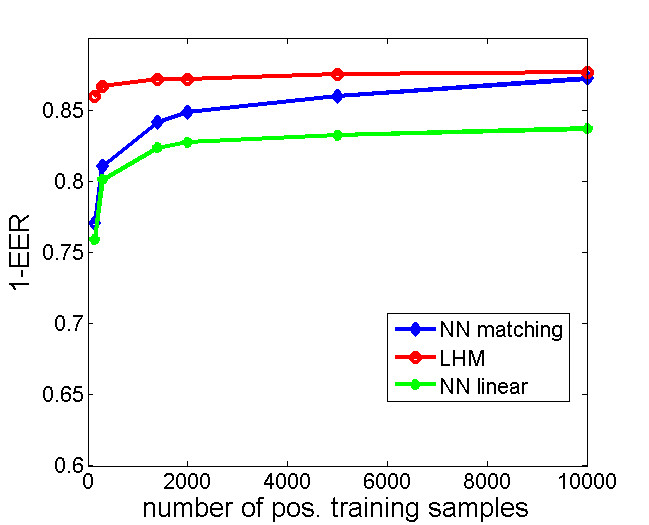
\includegraphics[width=0.49\linewidth]{pairs_binary_new.png}
  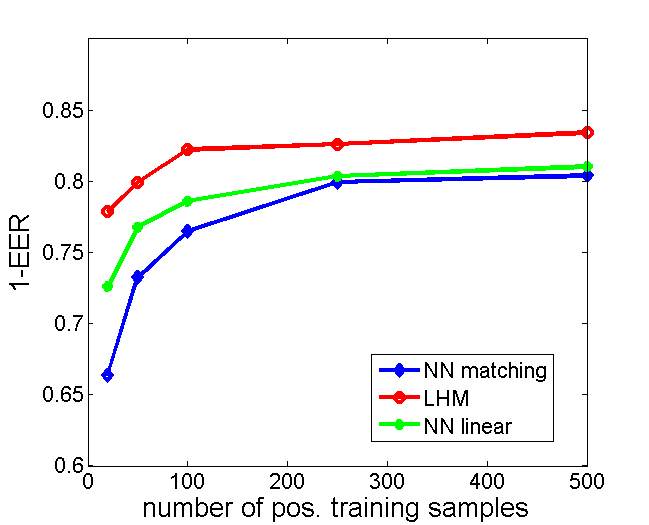
\includegraphics[width=0.49\linewidth]{transfer_binary_new.png}
  \caption{Binary imbalanced classification: left -- the ``best-case'' transfer learning setting, right -- the ``worst-case'' transfer learning  setting.} %The plots show the average (over 5 binary problems) 1-EER for LHM and NN as a function of positive training size: 140, 300, 1400, 2000, 1000(all) samples.} The accuracy of NN is averaged over 50 random initializations.}
  \label{fig:binary}
\end{figure}

\subsection{Hinge-Minimax Training in Deep Architecture}\label{sec:cifar_ex}
In the following experiments, we show that LHM classifier can be combined with CNN via transfer learning. Specifically, we test the LHM classifier on top of the pre-trained CNN feature extraction in imbalanced binary problems and in multi-class tasks with a small number of labeled examples.

We explore the following transfer learning settings. The first setting refers to the \textbf{best case} scenario in which the source and the target classification tasks operate on the \emph{same} set of features but differ in the classification problem. The second setting refers to the \textbf{worst case} scenario for the transfer learning where the source and the target classification problems \emph{share very little similarity}.  The ``worst case'' scenario is very common in practice, as many classification tasks do not have a large, comprehensive training set (such as ImageNet (\cite{imagenet_cvpr09}) in object recognition) to be used in transfer learning. No good solution currently exists for such problems.

We used the CIFAR-10, composed of 10 categories (airplane, automobile, bird, cat, deer, dog, frog, horse, ship, and truck) as the source problem. Specifically, we trained the LeNet model implemented in MatConvNet~\cite{vedaldi15matconvnet} on CIFAR-10. Then we removed the last fully-connected layer and the soft-max and used this trimmed network as a feature extractor which converts images to a $64$-dimensional feature vectors.

For the best case transfer learning, we defined a new set of classes by coupling $i$ and $i+5$ indexes of CIFAR-10 classes. CNN trained on CIFAR-10 maps individual classes to linearly separable sub-spaces, thus using pairs of classes as a target classification problem makes it non-linear. Consequently, we get a new classification problem over the same space of features.

For the worst case transfer learning, we picked a subset of 5 classes (train, bottle, cattle, forest, and sweet peppers) from the CIFAR-100, which do not overlap (in their visual appearance) with the CIFAR-10 categories, to be the target classification task. CIFAR-10 data set is not rich enough to enable learning of features that can be used for an arbitrary category, thus we believe that such setting is especially difficult.


We tested the LHM binary and multi-class classifiers in the best and the worst case transfer learning scenarios and compared their performance to two baselines. One is an NN with a single fully connected  layer and the cross-entropy loss (NN linear) and the other is the NN with the architecture matching the LHM model (NN matching).  We repeated each experiment 50 times over different random subsets of training samples and random initialization of NN and averaged the results.

\begin{figure}[h]
\center
  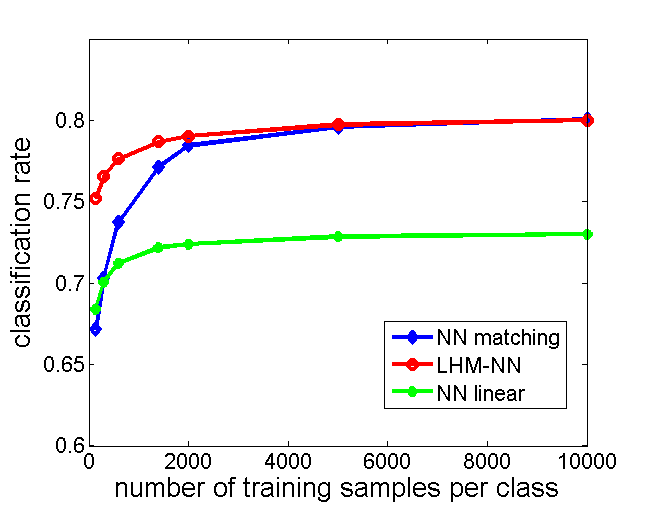
\includegraphics[width=0.49\linewidth]{mc_pairs_new.png}
  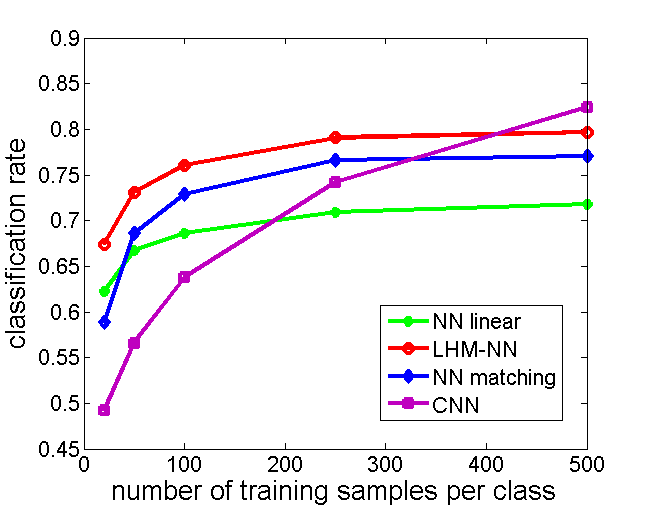
\includegraphics[width=0.49\linewidth]{mc_cifar100_new.png}
  \caption{Multi-class classification: left -- the ``best-case'' transfer learning  setting, right -- ``worst-case'' transfer learning  setting.}
  \label{fig:mc}
\end{figure}

\subsubsection{Binary Imbalanced Setting}
\noindent\textbf{The ``Best Case'' Transfer Learning:}
We trained binary classifiers for pairs of classes from CIFAR-10 using imbalanced training sets, in which the negative class included all samples from all other classes (40,000 examples) and the positive class included a varying number of samples (140, 300, 600, 1400, 2000, 5000-all). This resulted in imbalance ratios from 1:256 to 1:4.

LHM model was trained with 2 hidden components and 3 hyperplanes per component. The matching NN mimicked the configuration of LHM model, but the weights were allowed to change in training.  Figure~\ref{fig:binary}-left shows the 1-EER (averaged over 5 classification problems) of the LHM classifier and the two NN baselines as a function of the positive training sample size.


\noindent\textbf{The ``Worst Case'' Transfer Learning for Binary Imbalanced Problems:}
Since the number of samples per class in CIFAR-100 is significantly smaller, this experiment tests the robustness to imbalanced training data and to a small number of examples. We varied the size of the positive training set between 20, 50, 100, 250, 500(all) samples and we used all 2,000 samples of other classes as the negative training set. We compared the LHM model trained with 2 hidden components and  2 hyperplanes per component to NN baselines. Figure~\ref{fig:binary}-right shows the 1-EER of the classifiers averaged over 5 classification problems as a function of the positive training set size.

%In both setting the LHM model showed much better robustness to the size of the positive training set than the NN with matching architecture.

\subsubsection{Multi-Class Setting}
\noindent\textbf{The ``Best Case'' Transfer Learning:}
We mapped the LHM binary classifiers trained for 5 pairs of categories to a multi-class NN as described in Section~\ref{sec:mc_nn}. We fine-tuned the weights with a very fast training (just a handful of epochs, while training from scratch requires two orders of magnitude more training epochs). Figure~\ref{fig:mc}-left shows the accuracy of the LHM models mapped to a multi-class NN (LHM-NN) with the two baseline NNs as a function of the size of the training set.

\noindent\textbf{The ``Worst Case'' Transfer Learning for Multi-Class Problems:}
We mapped the LHM binary classifiers trained for the 5 categories from CIFAR-100 (using CIFAR-10 features) to a multi-class NN and fine-tuned the weights with a small number of epochs.

To test the complexity of the transfer learning problem we also trained a CNN (LeNet model implemented in MatConvNet (\cite{vedaldi15matconvnet})) on the target problem. We hoped that due to the small size of the target classification problem, 500 training examples per class would  yield relatively good accuracy. Figure~\ref{fig:mc}-right compares the accuracy of LHM-NN, two baseline NNs, and CNN (trained from scratch) as a function of the training sample size. It shows that CNN trained on the target problem is indeed the best as it succeeds to learn features specific for the task, but its accuracy drops very abruptly when the number of training samples becomes smaller. This suggests that when the number of training examples is small, using transfer learning even in a such difficult setting is a better solution than training a CNN from scratch.

The results in Figures \ref{fig:binary} and \ref{fig:mc} show that the NN models either heavily overfit when the number of  training samples is small (NN matching) or they are not expressive enough when the number of training samples increases (NN linear). LHM classifiers are expressive enough to learn from a large set of examples and are more robust to overfitting when the number of examples is small.


%Our experiments for multi-class problems show that LHM-NN is the best performing classifier when the number of labeled samples is small.  %The benefit of LHM-NN can be explained by its ability to incorporate unlabeled data into the training.

\section{Training Efficiency}
Another advantage of LHM-NN is its training efficiency. A class-specific LHM model converges in 5-10 iterations. Its training time primarily depends on the number of positive samples and the dimension. The negative samples are used to estimate the mean and covariance of the background. The initial estimation (which involves a large number of samples) is done only once and used for all classes. Since the probability of the negative class is evaluated inside the positive region using false positives, the number of which drops very fast, the estimation time of the mean and covariance during the training is negligible. Training of a binary classifier per class is independent of other classes, thus their training can be done in parallel. Finally, the fine-tuning of the multi-class network after mapping is very fast, due to the initialization of all layers (using supervized learning): feature extraction layers with pre-trained CNN and classifier's layers with LHM models.

The LHM-NN is also beneficial for the problems in which classes are dynamically added or removed from the classification task. Adding a class requires training a single binary classifier and fast fine-tuning; removing a class requires only fine-tuning.
\section{Conclusions and Future Work}
We proposed an efficient method for learning an intersection of finite number of hyperplanes which combines the hinge-risk (for the small number of positive data) with the background risk, based on the ``minimax bound'' (for a large number of negative data points) and derived a generalization bound for the mixed risk. We showed that the proposed classifier yields results comparable to the popular non-linear classifiers, but at much lower (order of magnitude) computational cost of classification. %The natural extension are multi-class learning for $K$ hyperplanes and a combination %of structured-hinge and minimax risks
%

We generalized this model to a non-convex classifier (Latent Hinge-Minimax classifier), which discovers the hidden components in the positive class and separates them from the negative class with the intersections of positive half spaces. The main advantage of this classifier is its ability to incorporate unlabeled data in training which improves the robustness to imbalanced sets.

We showed that for multi-class tasks, class-specific LHM models can be mapped to a multi-class NN with matching architecture requiring only a few iterations of fine-tuning. Finally, the showed that LHM architecture can be integrated with CNN features via transfer learning. The entire training procedure is very efficient. Our experiments showed that such classifiers are much more robust to the number of labeled training samples than the equivalent NNs.

This work cay be extended in various directions. A lower Rademacher complexity was shown for the k-fold maxima of hyperplanes in~\cite{Kontorovich18}. We plan to extend this result to the maximum over hinge losses and improve the generalization bound for the positive sample. Structured output learning have had an impact on machine vision and can be applied to this framework while improving the multiclass procedure. Another direction is devising a unified probabilistic framework to include both the hinge-loss and background-loss. Also, extensions of Marshall-Olkin theorem to non-convex sets might have a significant impact on robust deep learning methods.


\vskip 0.2in
\bibliography{hinge_minimax}

\end{document} 